% Options for packages loaded elsewhere
\PassOptionsToPackage{unicode}{hyperref}
\PassOptionsToPackage{hyphens}{url}
%
\documentclass[
  portuguese,
  ]{book}
\usepackage{lmodern}
\usepackage{amsmath}
\usepackage{ifxetex,ifluatex}
\ifnum 0\ifxetex 1\fi\ifluatex 1\fi=0 % if pdftex
  \usepackage[T1]{fontenc}
  \usepackage[utf8]{inputenc}
  \usepackage{textcomp} % provide euro and other symbols
  \usepackage{amssymb}
\else % if luatex or xetex
  \usepackage{unicode-math}
  \defaultfontfeatures{Scale=MatchLowercase}
  \defaultfontfeatures[\rmfamily]{Ligatures=TeX,Scale=1}
\fi
% Use upquote if available, for straight quotes in verbatim environments
\IfFileExists{upquote.sty}{\usepackage{upquote}}{}
\IfFileExists{microtype.sty}{% use microtype if available
  \usepackage[]{microtype}
  \UseMicrotypeSet[protrusion]{basicmath} % disable protrusion for tt fonts
}{}
\makeatletter
\@ifundefined{KOMAClassName}{% if non-KOMA class
  \IfFileExists{parskip.sty}{%
    \usepackage{parskip}
  }{% else
    \setlength{\parindent}{0pt}
    \setlength{\parskip}{6pt plus 2pt minus 1pt}}
}{% if KOMA class
  \KOMAoptions{parskip=half}}
\makeatother
\usepackage{xcolor}
\IfFileExists{xurl.sty}{\usepackage{xurl}}{} % add URL line breaks if available
\IfFileExists{bookmark.sty}{\usepackage{bookmark}}{\usepackage{hyperref}}
\hypersetup{
  pdftitle={Apontamentos de física},
  pdfauthor={Ricardo Cabeças},
  pdflang={pt},
  hidelinks,
  pdfcreator={LaTeX via pandoc}}
\urlstyle{same} % disable monospaced font for URLs
\usepackage{longtable,booktabs}
\usepackage{calc} % for calculating minipage widths
% Correct order of tables after \paragraph or \subparagraph
\usepackage{etoolbox}
\makeatletter
\patchcmd\longtable{\par}{\if@noskipsec\mbox{}\fi\par}{}{}
\makeatother
% Allow footnotes in longtable head/foot
\IfFileExists{footnotehyper.sty}{\usepackage{footnotehyper}}{\usepackage{footnote}}
\makesavenoteenv{longtable}
\usepackage{graphicx}
\makeatletter
\def\maxwidth{\ifdim\Gin@nat@width>\linewidth\linewidth\else\Gin@nat@width\fi}
\def\maxheight{\ifdim\Gin@nat@height>\textheight\textheight\else\Gin@nat@height\fi}
\makeatother
% Scale images if necessary, so that they will not overflow the page
% margins by default, and it is still possible to overwrite the defaults
% using explicit options in \includegraphics[width, height, ...]{}
\setkeys{Gin}{width=\maxwidth,height=\maxheight,keepaspectratio}
% Set default figure placement to htbp
\makeatletter
\def\fps@figure{htbp}
\makeatother
\setlength{\emergencystretch}{3em} % prevent overfull lines
\providecommand{\tightlist}{%
  \setlength{\itemsep}{0pt}\setlength{\parskip}{0pt}}
\setcounter{secnumdepth}{5}

%\usepackage[latin9]{inputenc}
%\usepackage[portuguese]{babel}
\usepackage[top=2cm,bottom=4cm,left=2cm,right=2cm]{geometry}
\usepackage{booktabs}
\usepackage{tikz}
\usepackage{amsmath}
\usepackage{fancyhdr}
%\usepackage[demo]{graphicx}
\usepackage{caption}
\usepackage{subcaption}
\usepackage{setspace}

\setstretch{1.5}
\pagestyle{fancy}
\fancyhead{}
%\fancyhead[RO,LE]{Capítulo \thechapter}
\fancyfoot{}

\fancyfoot[CO]{\thepage}
\fancyfoot[CE]{\thepage}
\newcommand{\dd}[1]{\mathrm{d}#1}
%\fancyfoot[CO,RE]{Author Name}
\ifxetex
  % Load polyglossia as late as possible: uses bidi with RTL langages (e.g. Hebrew, Arabic)
  \usepackage{polyglossia}
  \setmainlanguage[]{portuguese}
\else
  \usepackage[shorthands=off,main=portuguese]{babel}
\fi
\ifluatex
  \usepackage{selnolig}  % disable illegal ligatures
\fi
\usepackage[]{natbib}
\bibliographystyle{apalike}

\title{Apontamentos de física}
\author{Ricardo Cabeças}
\date{2021-12-02}

\begin{document}
\maketitle

{
\setcounter{tocdepth}{1}
\tableofcontents
}
\hypertarget{unidades-grandezas-e-anuxe1lise-dimensional}{%
\chapter{Unidades, grandezas e análise dimensional}\label{unidades-grandezas-e-anuxe1lise-dimensional}}

\hypertarget{velocidade-da-luz}{%
\section{Velocidade da luz}\label{velocidade-da-luz}}

Quando observamos e medimos fenómenos da nossa realidade, tentamos atribuir números às quantidade físicas com a maior precisão possível. Por exemplo, queremos detemrinar a velocidade da luz, que pode ser calculada dividindo a distância percorrida por um raio de luz pelo tempo que este a demora a percorrer,

\[veloc.da\ luz=\frac{dist.}{tempo}\]

Em 1983 a \(\textit{General Conference on Weights and Measures}\) definiu a velocidade da luz como sendo

\[c=299792458metros/segundo\]
Este número foi escolhido para corresponder à medição da velocidade da luz feita com maior precisão, dentro da incerteza experimental.

\hypertarget{sistema-internacional}{%
\section{Sistema Internacional}\label{sistema-internacional}}

As três quatidades, tempo, distância e velocidade da luz, estão directamente interligadas. Que quantidades devemos considerar como ``bases'' e quais são as quatidades ``derivadas''? Por exemplo, serão a distância e o tempo quantidades base enquanto a velocidade é uma quantidade derivada?

A resposta a esta questão é dada por convenção. O sistema básico de unidades usado em ciencia e tecnologia nos dias de hoje é o ``\emph{Système International}'' (SI). Consite em sete quantidades base e a suas unidades correspondentes.

\begin{longtable}[]{@{}cc@{}}
\toprule
Quantidade base & Unidade base\tabularnewline
\midrule
\endhead
distância & metro (m)\tabularnewline
massa & kilograma (kg)\tabularnewline
tempo & segundo (s)\tabularnewline
currente eléctrica & ampere (A)\tabularnewline
temperatura & Kelvin (K)\tabularnewline
quantidade de uma substância & mole (mol)\tabularnewline
intensidade luminosa & candela (cd)\tabularnewline
\bottomrule
\end{longtable}

\hypertarget{o-reluxf3gio-atuxf3mico-e-a-definiuxe7uxe3o-de-segundo}{%
\section{O relógio atómico e a definição de segundo}\label{o-reluxf3gio-atuxf3mico-e-a-definiuxe7uxe3o-de-segundo}}

Na obra \(\textit{Philosophiae Naturalis Principia Mathematica}\), Isaac Newton destinguiu o tempo para uma determinada duração e o tempo absoluto,

``\emph{Absolute true and mathematical time, of itself and from its own nature, flows equably without relation to anything external, and by another name is called duration: relative, apparent, and common time, is some sensible and external (whether accurate or unequable) measure of duration by means of motion, which is commonly used instead of true time; such as an hour, a day, a month, a year.}''

O desenvolvimento de relógios baseados em oscilações atômicas permitiu medidas de tempo com precisão na ordem de 1 parte em 10\(^{14}\), correspondendo a erros de menos de um microssegundo (um milionésimo de segundo) por ano. Dada a incrível precisão dessa medida e evidência clara de que os melhores cronometristas disponíveis eram de natureza atómica, o segundo (s) foi redefinido em 1967 pelo Comitê Internacional de Pesos e Medidas como um certo número de ciclos de radiação eletromagnética emitidos por átomos de césio quando fazem transições entre dois estados quânticos designados:

``\emph{Um segundo é a duração de 9192631770 periodos de radiação correspondentes à transição entre dois níveis hiperfinos do estádo fundamental do átomo de césio 133}''

\hypertarget{o-metro}{%
\section{O metro}\label{o-metro}}

O metro foi originalmente definido como 1/10.000.000 do arco que tem origem no Equador, segue ao longo do meridiano até ao Pólo Norte, passando por Paris. Para auxiliar na calibração e facilitar a comparação, o metro foi redefinido em termos de uma escala de comprimento gravada numa barra de platina preservada em Paris. õAssim que o laser começou a ter uma utilização mais comum, o metro foi redifinido pela \emph{17ª Conférence Générale des Poids et Mèsures (CGPM)} em 1983 para uma determinada quantidade de comprimentos de onda de um laser monocromático particular.

``\emph{O metro é a distancia percorrida pela luz no vácuo durante o intervalo de tempo de 1/299792458 segundos}''

\textbf{Exemplo:} O ano luz é a distância que a luz percorre num ano. Quantos metros percorre a luz num ano?

\textbf{Solução:} Usando a relação \[dist. = (veloc. \ da\  luz) . (tempo)\], um ano luz corresponde a uma distância. Como a velocidade da luz é dada em termos de metros por segundo, precisamos de saber quantos segundos existem num ano. Podemos fazer isto convertendo unidades. Sabemos que
\[1\ ano\ = 365.25\ dias,1\ dia=24\ horas,1\ hora=60\ minutos,\ 1\ minuto=60\ segundos\]

Fazendo os cálculos sabemos que o número de segundos num ano é de

\[1ano=(365.25\ dias)(\frac{24\ horas}{1\ dia})(\frac{60\ min}{1\ hora})(\frac{60\ s}{1\ min})=31557600\ s\]

Entao, a distância percorrida num ano é

\[1al=(\frac{299792458}{1s})(\frac{31557600}{1ano})(1ano)=9,461\times10^{15}m\]

A distância da estrela mais próxima, Alpha Centauri, é de três anos luz

\hypertarget{a-massa}{%
\section{A massa}\label{a-massa}}

A unidade de massa, o quilograma (kg), continua a ser a única unidade base no Sistema Internacional de Unidades (SI) que ainda está definido em termos de um artefato físico, conhecido como ``Protótipo Internacional do Quilograma Padrão''. O protótipo foi feito em 1879 por George Matthey sob a forma de um cilindro de 39 mm de altura e 39 mm de diâmetro, composto por uma liga de 90\% de platina e 10\% de irídio. O protótipo internacional é mantido no \(\textit{Bureau International des Poids et Mesures (BIPM)}\) em Sevres, França, nas condições especificadas pela 1ª Conferência Geral de Poesias e Misas (CGPM) em 1889, quando sancionou o protótipo e declarou: ``Este protótipo será doravante considerado a unidade de massa''. O protótipo é mantido num cofre com seis cópias oficiais.

\textbf{Exemplo 2: The International Prototype Kilogram} Determine o tipo de forma e dimensões que o protótipo do quilograma de platina-irídio terá, de modo a ter a menor área de superfície para um determinado volume. O quilograma padrão é uma liga de 90\% de platina e 10\% de irídio. A densidade da liga é \(\rho = 21,56g.cm^{-3}\). Podem-se considerar as seguintes questões:

\begin{itemize}
\item
  Existe alguma razão para que a área de superfície do quilograma padrão seja importante?
\item
  qual é a densidade que se deve usar?
\item
  qual é a forma (cubo, esfera, cilindro, etc) que tem a menor area de superficie para um dado volume?
\item
  porquê a escolha de um cilindro?
\end{itemize}

\textbf{Solução:} O quilograma padrão é uma liga de 90\% platina e 10\% irídium. A densidae da plantina ´é de \(\rho = 21,45 g.cm^{-3}\) e a densidade do irídium é de \(\rho = 22,55 g.cm^{-3}\). Então a densidade do quilograma padrão é, \[\rho = 21,56g.cm^{-3}\] eo volume é

\[V=m/\rho\cong1000g/22g.cm^{-3}=46,38cm^{3} \]

A corrosão afectaria a mass através de reacções quimicas; a platina e o irídium foram escolhidos para a composição do quiligrama padrão por resistirem à corrosão.

Para minimizar ainda mais a corrosão, a forma deve ser escolhida para ter a menor área de superfície. Idealmente, esta seria uma esfera, mas como as esferas rolam facilmente, tornam-se impraticáveis, enquanto que os cilindros têm superfícies planas que os mantém fixos. O volume para um cilindro é dado por

\[V=\pi r^2h\]

A área de superfície pode ser expressa em função de \(r\)

\[A=2\pi r^2+2\pi rh=2\pi r^2+\frac{2V}{r}\]

Para encontrar a menor área de superfície, minimizamos a área em função do raio, \(r\)

\[\frac{dA}{dr}=4\pi r - \frac{2V}{r^2}\]

ficamos com

\[r^3=\frac{V}{2\pi}=\frac{\pi r^2 h}{2 \pi}\]

Assim podemos concluir que o raio é metade da altura

\[r=\frac{h}{2}\]

Para o quilograma padrão, o raio é

\[r=\Big(\frac{V}{2\pi}\Big)^{1/3}=\Big(\frac{46,38\ cm^3}{2\pi}\Big)^{1/3}\cong1,95\ cm\]

\hypertarget{definiuxe7uxe3o-alternativa-de-massa}{%
\subsection{Definição alternativa de massa}\label{definiuxe7uxe3o-alternativa-de-massa}}

Devido ao facto do protótipo do quilograma ser um objecto físico, existem problemas intrinsecos associados, como por exemplo, o protótipo ser danificado ou destruído. O protótipo ganha atomos devido ao ambiente que o rodeia e à sua manutenção. Este ganho de ´átomos traduz-se numa taxa de aproximadamente \(1\mu g/ano\) (\(1\mu g = 1\times10^{-6}g\))

Várias aproximações para definir a unidade da mass est\textasciitilde ão actualmente a serem exploradas. Um possibilidade é definir o kg como um número fixo de átomos, relacionando o kg com massa atómica. O silicone é um bom candidato porque pode ser criado em laboratório, de maneira controlada.

\textbf{Exemplo 3: Massa de um cristal de silicone}

Uma determinada quantidade de silicone tem um vomule \(V_0\) e contém \(N_0\) átomos. O número de moléculas numa mole de uma substância é dada pela constante de Avogadro \(N_A=6,0221415\times10^{23}\ mole^{-1}\). A massa molar do silicone é dada por \(M_{molar}\). Qual é a massa \(m\) de um determinado volume \(V\) em função de \(V_0\), \(N_0\), \(V\), \(M_{molar}\) e \(N_A\)

\textbf{Solução:} A massa \(m_0\) de uma unidade de silicone ´é a densidade \(\rho\) do silicon a multiplicar pelo volume da unidade de silicone \(V_0\),

\[m_0=\rho V_0\]

O número de moles na unidade é a massa total da unidade, \(m_0\), a dividir pela massa molar \(M_{molar}\),

\[n_0=m_0/M_{molar}=\rho V_0/M_{molar}\]
O nºumero de átomos na unidade é o numero de moles, \(n_0\), vezes a contaste de Avogadro, \(N_A\),

\[N_0=n_0N_A=\frac{\rho V_0 N_A}{M_{molar}}\]
A densidade do cristal está relacinada com a massa \(m\) do cristal dividida pelo volume \(V\) do cristal,

\[\rho=m/V\]
Então o número de átomos poder expresso por,

\[N_0=\frac{mV_0N_A}{VM_{molar}}\]
e a massa do cristal é

\[m=\frac{M_{molar}}{N_A}\frac{V}{V_0}N_0\]

A massa molar e o volume do cristal podem ser medidos directamente. Olhando para a ultima equação podemos verificar que \(M_{molar}/N_A\) é a massa de um átomo e que \((V/V_0)N_0\) é o número de átomos no volume. Esta aproximação está limitada ao problema da medição da constante de Avogadro, \(N_A\), com uma incerteza de \(1\) parte em \(10^8\), que é equivalente à incerteza da anteriaor definição de quilograma

\hypertarget{dimuxeansuxf5es-de-quantidades-comuns}{%
\section{Dimênsões de quantidades comuns}\label{dimuxeansuxf5es-de-quantidades-comuns}}

Muitas quantidades físicas são derivadas de quantidades base a partir de relações algébricas que definem a relação física entre essas quantidades. A dimensão da quantidade derivada é escrita como uma potência da dimensão da quantidade base.

Por exemplo, a velocidade é uma quantidade derivada e a sua dimensão é dada pela ralação

\[dim. veloc.=\frac{dist.}{tempo}=D.T^{-1}\]

onde D = distância, T = tempo

A força também é uma quantidade derivada e tem dimensão

\[dim. força =\frac{(massa)(dim.\ veloc.)}{tempo}\]

onde M = massa. Podemos então expressar a força em termos de massa, distância e tempo pela relação

\[dim. força=\frac{(massa)(dist.)}{(tempo)^2}=M.D.T^{-2}\]

A energia cinética (EC) também é uma quantidade derivada

\[dim. EC=(massa).(dim.\ veloc.)^2\]

que em termos de massa, distância e tempo é

\[dim. EC=\frac{(massa)(dist.)^2}{(tempo)^2}=M.D^2.T^{-2}\]

O trabalho deriva da força e da distância

\[dim. trab.=(dim.\ força)(dist.)\]

que em termos das dimensões fundamentais é

\[dim. trab.=\frac{(massa)(dist.)^2}{(tempo)^2}=M.D^2.T^{-2}\]

Então, podemos afirmar que trabalho e energia cinética têm as mesmas dimensões

\begin{table}

\caption{\label{tab:unnamed-chunk-2}Dimensões de algumas quantidades}
\centering
\begin{tabular}[t]{l|l|l}
\hline
Quantidade & Dimensão & unidade\\
\hline
Ângulo & sem dimensão & radianos\\
\hline
Área & D\textasciicircum{}2\textasciicircum{} & m\textasciicircum{}2\textasciicircum{}\\
\hline
Volume & D\textasciicircum{}3\textasciicircum{} & m\textasciicircum{}3\textasciicircum{}\\
\hline
Frequência & T\textasciicircum{}-1\textasciicircum{} & s\textasciicircum{}-1\textasciicircum{} = Hz\\
\hline
Velocidade & D.T\textasciicircum{}-1\textasciicircum{} & m.s\textasciicircum{}-1\textasciicircum{}\\
\hline
Aceleração & D.T\textasciicircum{}-2\textasciicircum{} & m.s\textasciicircum{}-2\textasciicircum{}\\
\hline
Velocidade Angular & T\textasciicircum{}-1\textasciicircum{} & rad.s\textasciicircum{}-1\textasciicircum{}\\
\hline
Aceleração Angular & T\textasciicircum{}-2\textasciicircum{} & rad.s\textasciicircum{}-2\textasciicircum{}\\
\hline
Densidade & M.D\textasciicircum{}3\textasciicircum{} & kg.m\textasciicircum{}-3\textasciicircum{}\\
\hline
Momento & M.D.T\textasciicircum{}-1\textasciicircum{} & kg.m.s\textasciicircum{}-1\textasciicircum{}\\
\hline
Momento Angular & M.D\textasciicircum{}2\textasciicircum{}.T\textasciicircum{}-1\textasciicircum{} & kg.m\textasciicircum{}2\textasciicircum{}.s\textasciicircum{}-1\textasciicircum{}\\
\hline
Força & M.D.T\textasciicircum{}-2\textasciicircum{} & kg.m.s\textasciicircum{}-2\textasciicircum{} = N\\
\hline
Trabalho, Energia & M.D\textasciicircum{}2\textasciicircum{}.T\textasciicircum{}-2\textasciicircum{} & kg.m\textasciicircum{}2\textasciicircum{}.s\textasciicircum{}-2\textasciicircum{} = J\\
\hline
Torque & M.D\textasciicircum{}2\textasciicircum{}.T\textasciicircum{}-2\textasciicircum{} & kg.m\textasciicircum{}2\textasciicircum{}.s\textasciicircum{}-2\textasciicircum{}\\
\hline
Potência & M.D\textasciicircum{}2\textasciicircum{}.T\textasciicircum{}-3\textasciicircum{} & kg.m\textasciicircum{}2\textasciicircum{}.s\textasciicircum{}-3\textasciicircum{} = W\\
\hline
Pressão & M.D\textasciicircum{}-1\textasciicircum{}.T\textasciicircum{}-2\textasciicircum{} & kg.m\textasciicircum{}-1\textasciicircum{}.s\textasciicircum{}-2\textasciicircum{} = Pa\\
\hline
\end{tabular}
\end{table}

\hypertarget{anuxe1lise-dimensional}{%
\section{Análise dimensional}\label{anuxe1lise-dimensional}}

Existem muitos fenómenos na natureza que podem ser explicados através de simples relações entre os fenómenos observados

\textbf{Exemplo 4: Período de um pêndulo}

Consideremos um pêndulo simples constituído por uma massa, suspensa a partir de uma ponto fixo por um fio. Seja \(T_{período}\) o tempo que o pêndulo demora a completar um ciclo de ida e volta. Quais são as quantidades que definem o pêndulo e quais a quantidades que definem o seu movimento?

\textbf{Solução}

Que quantidades estão envolvidas? O comprimento do pêndulo \(l\), a massa de pêndulo \(m\), a aceleração gravítica \(g\) e a amplitude angular \(\theta_0\) são as quantidades que se podem relacionar com o pêndulo e o seu movimento. Será que incluímos todas as qualidades possíveis? Primeiro vamos trabalhar com as variáveis que listamos atrás e, caso seja necessário mais alguma variável, teremos que pensar um bocadinho mais!

O nosso problema é então encontrar uma função \(f\) tal que

\[T_{periodo}=f(l,m,g,\theta_0)\]

Primeiro, criamos uma lista das dimensões das quantidades como mostra a tabela seguinte. Escolhemos o conjunto: massa, comprimento e tempo, para usar como dimensões da base.

\begin{table}

\caption{\label{tab:unnamed-chunk-3}Dimensões das quantidade que podem descrever o período de um pêndulo}
\centering
\begin{tabular}[t]{l|l|l}
\hline
Nome da quantidade & Simbolo & Fórmula dimensional\\
\hline
tempo & t & T\\
\hline
comprimento do pêndulo & l & L\\
\hline
massa do pêndulo & m & M\\
\hline
aceleração gravítica & g & L.T\textasciicircum{}2\textasciicircum{}\\
\hline
amplitude angular & \textbackslash{}(\textbackslash{}theta\_0\textbackslash{}) & sem dimensão\\
\hline
\end{tabular}
\end{table}

A primeira observação é que a massa do pêndulo não pode entrar na relação, isto porque a nossa quantidade final não tem dimensão de massa e não existe outra quantidade que possa remover a dimensão de massa do pêndulo. Vamos focar-nos no comprimento do fio e na aceleração gravítica. Para eliminar o comprimento, estas quantidades devem dividir entre elas, para depois podermos igualar o \(T_{período}\) com uma variável de dimensão tempo. Escolhamos a combinação \(l/g\), as dimensões são

\[dim[l/g]=\frac{comprimento}{\frac{comprimento}{(tempo)^2}}=tempo^2\]

Temos então uma relação que nos diz que o tempo que o pêndulo demora a ir de uma extremidade da sua trajectória à outra extremidade é a raiz quadrada do rácio \(l/g\)
A fórmula candidata é

\[T_{período}\sim\Big(\frac{l}{g}\Big)^{1/2}\]

Como a amplitude angular não tem dimensão, pode ou não aparecer na equação. Podemos adicionar uma função \(y(\theta_0)\) não nossa equação, só para introduzir a amplitude angular, visto que a análise desta vai para além deste tópico. Assim a equação final fica

\[T_{período}=y(\theta_0)\Big(\frac{l}{g}\Big)^{1/2}\]

que para amplitudes muito pequenas \(y(\theta_0)=2\pi\),

\[T_{período}=2\pi\Big(\frac{l}{g}\Big)^{1/2}\]

\hypertarget{cinemuxe1tica-unidimuxeansional}{%
\chapter{Cinemática unidimênsional}\label{cinemuxe1tica-unidimuxeansional}}

A cinemática é a descrição matemática do movimento. O termo é derivado da palavra grega \emph{kinema}, que significa movimento. Para quantificar o movimento, um sistema de coordenadas matemáticas, chamado de sistema de referência, é usado para descrever espaço e tempo. Uma vez escolhido um sistema de referência, podemos introduzir os conceitos físicos de posição, velocidade e aceleração de forma matematicamente precisa. A Figura 4.1 mostra um Sistema de coordenadas cartesianas em uma dimensão com vetor unitário \(\widehat{i}\) apontando no sentido positivo do eixo das abcissas

\begin{figure}

{\centering 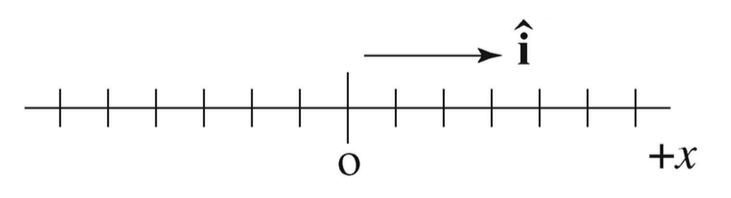
\includegraphics[width=0.6\linewidth]{img/1} 

}

\caption{Sistema cartesiano unidimênsional}\label{fig:img1}
\end{figure}

\hypertarget{posiuxe7uxe3o-intervalo-de-tempo-deslocamento}{%
\section{Posição, intervalo de tempo, deslocamento}\label{posiuxe7uxe3o-intervalo-de-tempo-deslocamento}}

\hypertarget{posiuxe7uxe3o}{%
\subsection{Posição}\label{posiuxe7uxe3o}}

Considere um objeto movendo-se em uma dimensão. Denotamos a coordenada de posição do centro de massa do objeto em relação à escolha de origem por x (t). A coordenada de posição é uma função do tempo e pode ser positiva, zero ou negativa, dependendo da localização do objeto. A posição tem direção e magnitude, e, portanto, é um vetor,

\[
\vec{x}(t)=x(t)\widehat{i}
\]

Denotamos a posição na origem em \(t=0\) por \(x_0=x(t=0)\). A unidade SI para a posição é o metro \([m]\)

\begin{figure}

{\centering 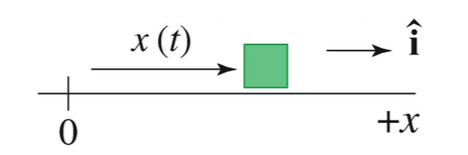
\includegraphics[width=0.4\linewidth]{img/2} 

}

\caption{Vector posição com referência à origem}\label{fig:img2}
\end{figure}

\hypertarget{intervalo-de-tempo}{%
\subsection{Intervalo de Tempo}\label{intervalo-de-tempo}}

Consideremos umintervalo de tempo fechado \([t_1,t_2]\). Caracterizamos este intervalo de tempo pela diferença dos limites desse intervalo tal que,

\[\Delta t=t_2-t_1\]

A unidade SI para os intervalos de tempo é o segundo \([s]\)

\hypertarget{deslocamento}{%
\subsection{Deslocamento}\label{deslocamento}}

Um mudança da massa no sistema de coordenadas entre os tempos \(t_1\) e \(t_2\) é tal que

\[\Delta\vec{x}=(x(t_2)-x(t_1))\vec{i}=\Delta x(t)\vec{i}\]

A \(\Delta \vec{x}\) podemos chamar de *deslocamento entre o tempo \(t_1\) e \(t_2\). O deslocamente é uma quantidade vectorial

\begin{figure}

{\centering 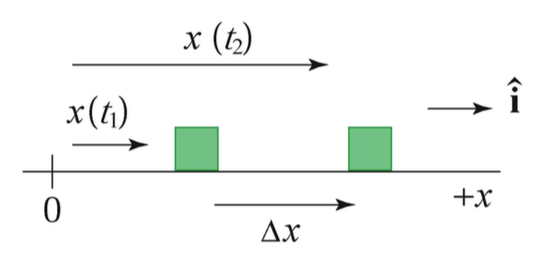
\includegraphics[width=0.4\linewidth]{img/3} 

}

\caption{Deslocamento de um objecto num intervalo de tempo é o vector resultante da diferença entre as posições}\label{fig:img3}
\end{figure}

\hypertarget{velocidade}{%
\section{Velocidade}\label{velocidade}}

Ao descrever o movimento de objetos, palavras como ``rapidez'' e ``velocidade'' são usadas em linguagem comum; No entanto, ao introduzir uma descrição matemática do movimento, precisamos definir estes termos com precisão. O nosso procedimento será definir quantidades médias para intervalos de tempo finitos e depois examinar o que acontece no limite, pois o intervalo de tempo torna-se infinitamente pequeno. Isto leva-nos ao conceito matemático de que a velocidade num instante no tempo é a derivada da posição em relação ao tempo.

\hypertarget{velocidade-muxe9dia}{%
\subsection{Velocidade média}\label{velocidade-muxe9dia}}

A componente da velocidade média, \(\overline{v_x}\), para um intervalo de tempo \(\Delta t\) ´é definido como o deslocamento \(\Delta x\) dividido pelo o intervalo de tempo \(\Delta t\),

\[\overline{v_x}=\frac{\Delta x}{\Delta t}\]

A unidade SI para a velocidade é o metro por segundo \([m.s^{-1}]\)

\hypertarget{velocidade-instantuxe2nea}{%
\subsection{Velocidade instantânea}\label{velocidade-instantuxe2nea}}

Considere um corpo movendo-se numa direção. Consideremos a coordenada de posição do corpo x(t), com a posição inicial \(x_0\) no tempo \(t = 0\). Consideremos o intervalo de tempo \([t, t + \Delta t]\). A velocidade média para o intervalo é a inclinação da linha que liga os pontos \((t, x (t))\)e \((t, x (t + \Delta t))\). O declive da recta é a mudança de posição sobre a mudança de tempo e é dada por

\[\overline{v_x}=\frac{\Delta x}{\Delta t}=\frac{x(t+ \Delta t)-x(t)}{\Delta t} \]

Vamos ver o que acontece com a velocidade média à medida que reduzimos o tamanho do intervalo de tempo. A inclinação da linha que liga os pontos \((t, x (t))\) e \((t, x (t + \Delta t)\) aproxima-se da inclinação da linha tangente para a curva \(x(t)\) no tempo \(t\).

\begin{figure}

{\centering 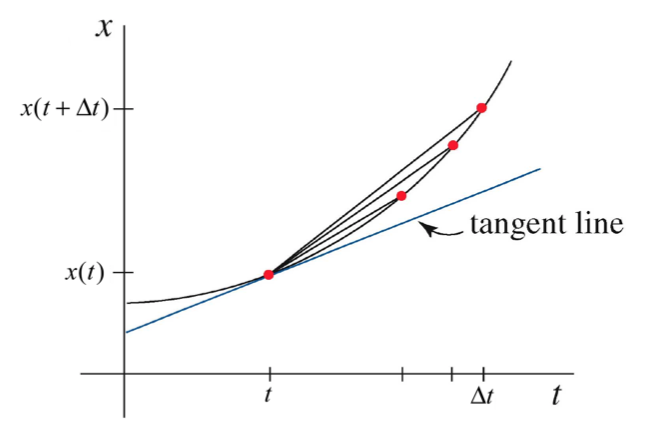
\includegraphics[width=0.4\linewidth]{img/4} 

}

\caption{Gráfico da posição vs. tempo que mostra a linha tangente no tempo $t$}\label{fig:img4}
\end{figure}

\hypertarget{velocidade-instantuxe2nea-1}{%
\subsection{Velocidade instantânea}\label{velocidade-instantuxe2nea-1}}

A componente do x da velocida de instantânea no tempo \(t\) é dada pelo declive a reta tangente à curva da posição vs.~tmepo no tmepo \(t\)

\[v_x(t)=\lim_{\Delta t \rightarrow0}{\overline{v_x}}=\lim_{\Delta t \rightarrow0}\frac{\Delta x}{\Delta t}= \lim_{\Delta t \rightarrow0} \frac{x(t+\Delta t)-x(t)}{\Delta t}=\frac{dx}{dt}\]

\hypertarget{acelerauxe7uxe3o}{%
\section{Aceleração}\label{acelerauxe7uxe3o}}

Devemos aplicar o mesmo procedimento físico e matemático para definir a aceleração, a taxa de mudança de velocidade. Consideremos primeiro como a velocidade instantânea muda ao longo de um intervalo de tempo e, em seguida, calculamos o limite à medida que o intervalo de tempo se aproxima de zero.

\hypertarget{acelerauxe7uxe3o-muxe9dia}{%
\subsection{Aceleração média}\label{acelerauxe7uxe3o-muxe9dia}}

A aceleração é a quantidade que mede uma mudança de velocidade num determinado intervalo de tempo. Suponhamos que durante um intervalo de tempo \(\Delta t\) um corpo sofre uma mudança de velocidade

\[\Delta \overrightarrow{v}=\overrightarrow{v}(t+\Delta t)-\overrightarrow{v}(t)\]

A mudança na componente do \(x\) da velocidade, \(\Delta v_x\), para o intervalo de tempo \([t,t+\Delta t]\) é então

\[\Delta v_x=v_x(t+\Delta t)-v_x(t)\]

A unidade SI para a aceleração média é o metro por segundo ao quadrado, \([m.s^{-2}]\)

\hypertarget{acelerauxe7uxe3o-instantuxe2nea}{%
\subsection{Aceleração instantânea}\label{acelerauxe7uxe3o-instantuxe2nea}}

Num gráfico da componente \(x\) da velocidade vs.~tempo, a aceleração média para um intervalo de tempo \(\Delta t\) é a inclinação da linha reta conectando os dois pontos \((t, v_x (t))\) e \((t +\Delta t, v_x (t +\Delta t))\). Para definir a componente \(x\) da aceleração instantânea no tempo \(t\), empregamos o mesmo argumento do limite que fizemos quando definimos a velocidade instantânea em termos da inclinação da linha tangente.

A componente \(x\) da aceleração instantânea no tmepo \(t\) é o limite do decliveda linnha tangente no instante \(t\) do gráfico da componente \(x\) da velocidade em função do tempo

\[a_x(t)=\lim_{\Delta \rightarrow 0}\overline{a_x}=\lim_{\Delta \rightarrow 0}\frac{(v_x(t+\Delta t)-v_x(t))}{\Delta t}=\lim_{\Delta \rightarrow 0}\frac{\Delta v_x}{\Delta t}=\frac{dv_x}{dt}\]

\begin{figure}

{\centering 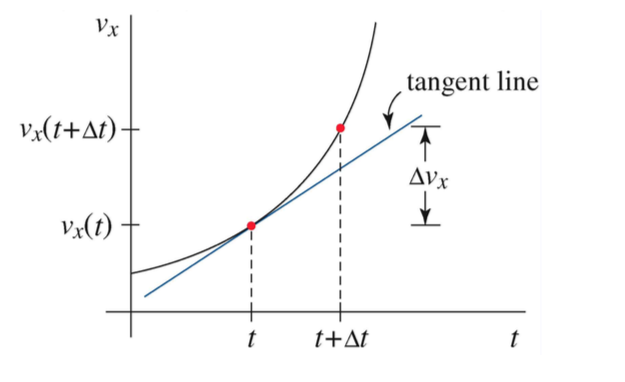
\includegraphics[width=0.5\linewidth]{img/5} 

}

\caption{Gráfico da velocidade vs. tempo que mostra a linha tangente no tempo $t$}\label{fig:img5}
\end{figure}

Como a velocidade é a derivada da posição em relação ao tempo, a componente \(x\) da aceleração é a segunda derivada da função de posição,

\[a_x=\frac{dv_x}{dt}=\frac{d^2x}{dt}\]

\hypertarget{vectores}{%
\chapter{Vectores}\label{vectores}}

\hypertarget{introduuxe7uxe3o-aos-vectores}{%
\section{introdução aos vectores}\label{introduuxe7uxe3o-aos-vectores}}

Certas quantidades físicas, como massa ou volume, têm apenas magnitude, ou seja, são representadas por um único valor. Os números que por si só podem representar estas quantidades, com as unidades apropriadas, são chamados de escalares. No entanto, existem outras grandezas físicas que têm magnitude e direcção: a magnitude pode aumentar ou diminuir, e a direção pode ser alterada. Estas quantidades podem ser adicionadas tendo em conta a direcção e a magnitude. A força é um exemplo de uma quantidade que actua numa determinada direcção com um determinada magnitude que se mede em newtons. Quando duas forças actuam sobre um objecto, a soma das forças depende da direção e da magnitude das duas forças. Posição, deslocamento, velocidade, aceleração, força, momento e torque são todas quantidades físicas que podem ser representadas matematicamente por vectores.

\hypertarget{propriedades-dos-vectores}{%
\section{Propriedades dos vectores}\label{propriedades-dos-vectores}}

Um vector é definido por uma direcção e uma magnitude. Normalmente usa-se o símbolo \(\vec{A}\) para representar um vector sendo que a magnitude do vector é \(|\vec{A}|\equiv A\). Geometricamente um vector pode ser representado por um seta que aponte para a direcção do vector, sendo o tamanho da seta a magnitude \(|\vec{A}|\).

\begin{figure}

{\centering 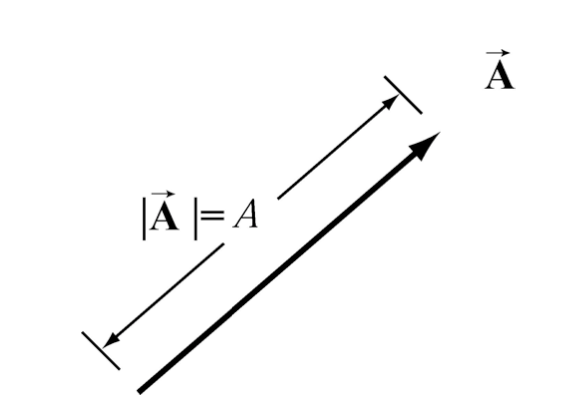
\includegraphics[width=0.5\linewidth]{img/6-vector} 

}

\caption{Representação de um vector}\label{fig:img6}
\end{figure}

\hypertarget{soma-de-vectores}{%
\section{Soma de vectores}\label{soma-de-vectores}}

Os vectores podem ser somados. Sejam \(\vec{A}\) e \(\vec{B}\) dois vectores, podemos definir um terceiro vector por \(\vec{C}=\vec{A}+\vec{B}\), onde \(\vec{C}\) é o vector resultante da soma entre \(\vec{A}\) e \(\vec{B}\). Para efectuar esta soma devemos desenhar o vector \(\vec{A}\) e colocar a cauda do vector \(\vec{B}\) na ponta do vector \(\vec{A}\) como mostra a figura \ref{fig:fig7} (esquerda). A seta que começa no início do \(\vec{A}\) e acaba na ponta do \(\vec{B}\) é definida como o vector adição \(\vec{C}=\vec{A}+\vec{B}\). Outra maneira equivalente de adicionar vectores é colocar o início dos vectores \(\vec{A}\) e \(\vec{B}\) no mesmo ponto, definindo assim os lados de um paralelogramo. O vector \(\vec{C}=\vec{A}+\vec{B}\) será a diagonal desse paralelogramo (figura \ref{fig:fig7} - direita)

\begin{figure}

{\centering 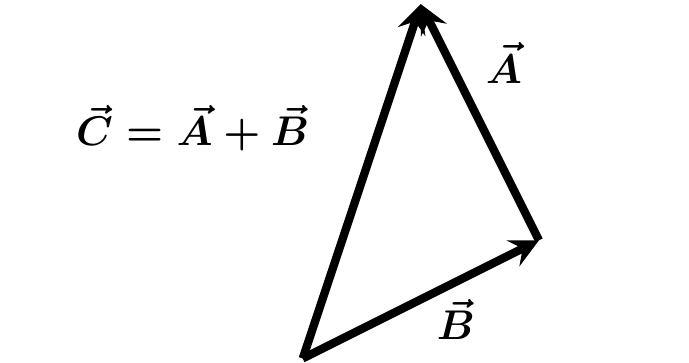
\includegraphics[width=0.9\linewidth]{Livro_files/figure-latex/fig7-1} 

}

\caption{Soma geométrica de vectores}\label{fig:fig7}
\end{figure}

A adição de vectores satisfaz as seguintes propriedades:

\begin{itemize}
\tightlist
\item
  \textbf{Comutativa -\textgreater{}} A ordem da adição dos vectores não interessa
\end{itemize}

\[\vec{B}+\vec{A}=\vec{A}+\vec{B}\]

\begin{itemize}
\tightlist
\item
  \textbf{Associativa -\textgreater{}} Quando se adiciona 3 vectores, não interessa a ordem por onde se começa
\end{itemize}

\[ (\vec{A}+\vec{B})+\vec{C}=\vec{A}+(\vec{B}+\vec{C})\]

\begin{itemize}
\tightlist
\item
  \textbf{Elemento identidade na adição de vectores -\textgreater{}} Existe um vector único, \(\vec{0}\), que actua como vector identidade para o vector adição. Para todos os vectores \(\vec{A}\)
\end{itemize}

\[\vec{A}+\vec{0}=\vec{0}+\vec{A}=\vec{A}\]

\begin{itemize}
\tightlist
\item
  \textbf{Elemento inverso para a adição de vectores -\textgreater{}} Para cada vector \(\vec{A}\), existe um vector inverso único
  \[(-1)\vec{A}\equiv-\vec{A}\]
  tal que
  \[\vec{A}+(-\vec{A})=\vec{0}\]
  O vector \(-\vec{A}\) tem a mesma magnitude que \(\vec{A}\), \(|\vec{A}|=|-\vec{A}|=A\), mas apontam para sentidos opostos (\ref{fig:fig8}).
\end{itemize}

\begin{figure}

{\centering 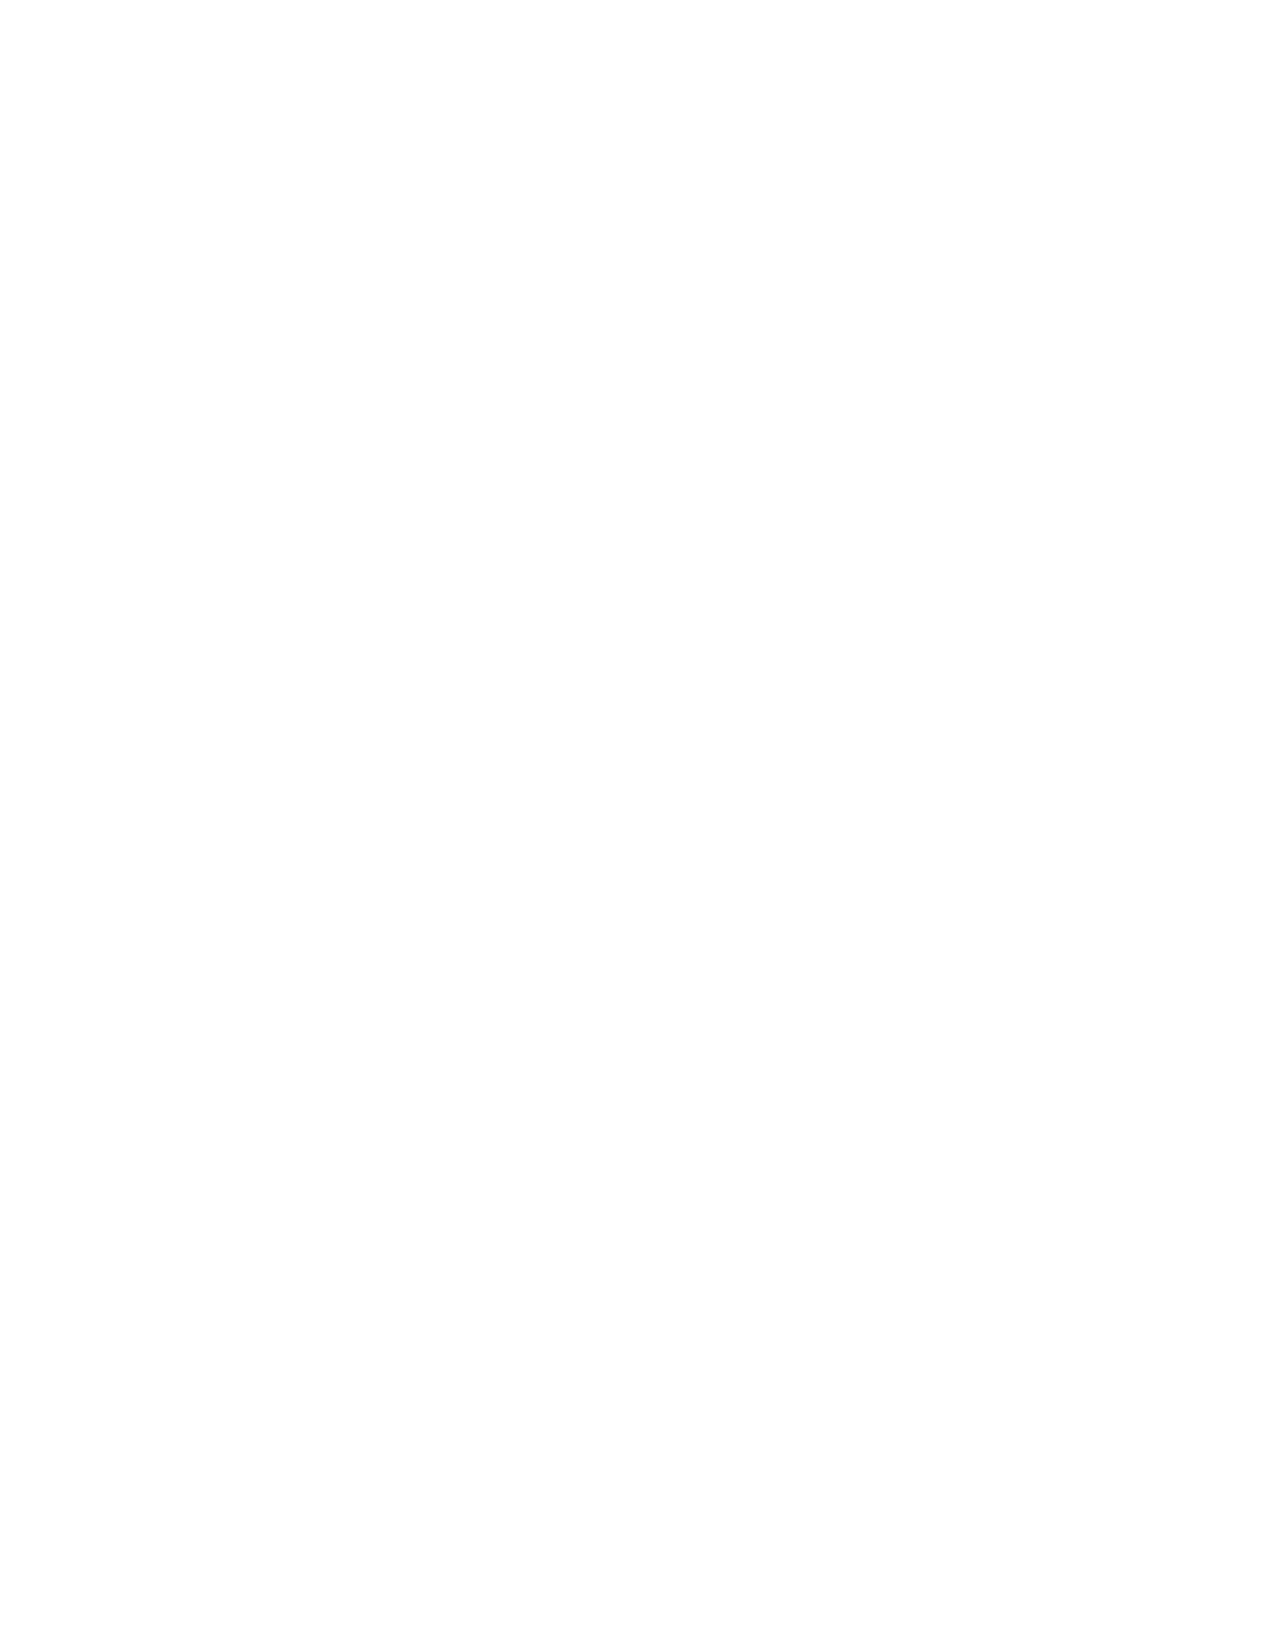
\includegraphics[width=0.9\linewidth]{Livro_files/figure-latex/fig8-1} 

}

\caption{Soma geométrica de vectores}\label{fig:fig8}
\end{figure}

\hypertarget{multiplicauxe7uxe3o-escalar-de-vectores}{%
\section{Multiplicação escalar de vectores}\label{multiplicauxe7uxe3o-escalar-de-vectores}}

Os vectores podem ser multiplicados por números reais. Seja \(\vec{A}\) um vector e \(c\) um número real positivo, a multiplicação de \(\vec{A}\) por \(c\) será um novo vector \(c\vec{A}\). A magnitude de \(c\vec{A}\) será \(c\) vezes a magnitude de \(\vec{A}\)

\[|c\vec{A}|=c|\vec{A}|\]

\begin{equation}
|c\vec{A}|=c|\vec{A}|
\label{eq:escvec}
\end{equation}

\hypertarget{lei-de-hooke}{%
\chapter{Lei de Hooke}\label{lei-de-hooke}}

Todos os materiais sólidos exibem um comportamento quando sujeitos a forças de compressão ou tracção. Se a relação entre a força aplicada e a deformação do material for linear, ou seja, se existir uma relação de proporcionalidade directa, diz-se que o material obedece à Lei de Hooke.

\textbf{Definição da Lei de Hooke:} Quando um material elástico sofre uma deformação devido a uma força de tracção ou de compressão, desenvolve-se uma força de pressão (força por unidade de área) que é proporcional à deformação relativa, ou alongamento unitário.

\begin{figure}

{\centering 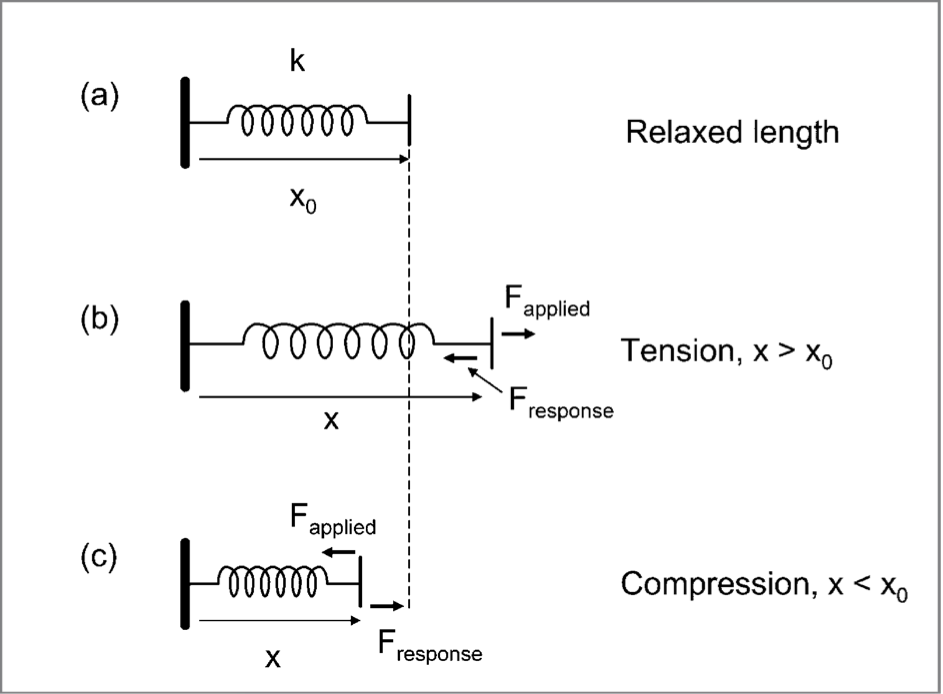
\includegraphics[width=0.5\linewidth]{img/lei_de_hooke_1} 

}

\caption{Modelo de mola para materiais elásticos (a) relaxado (b) sobre tensão (c) sobre compressão}\label{fig:img61}
\end{figure}

Na figura \ref{fig:img61} encontra-se um esquema que utiliza a analogia de uma mola elástica. Na posição x0, o material está no seu estado normal, sem sofrer a acção de uma força. Quando é exercida uma força de tracção (tension) o comprimento do material aumenta e passa a ser x. Quando o material sofre uma força de compressão (compression) o seu comprimento também se altera, diminuindo.
Em termos matemáticos esta relação exprime-se pela formula:

\[ F= -kx\]

onde F é a força aplicada, k é a constante elástica da mola e x é o deslocamento.
Num sólido, a força aplicada é distribuída pela superficie do sólido sobre a qual a força incide. Existe então uma relação entre a força aplicada e a área da superficie, a qual se designa por stress:

\[\sigma=\frac{F}{A}\]

Esta relação é directamente proporcional à deformação do material, se e só se o material obedecer à lei de Hooke.
A deformação relativa do material é dada por:

\[\epsilon=\frac{L-L_0}{L_0}\]

em que \(L_0\) é o comprimento original no material e \(L\) é o comprimento do material sob a acção da força aplicada.
Assim, a relação entre a força aplicada num material e o deslocamento (por compressão ou tracção, figura \ref{fig:img7} é dado por,

\[\frac{F}{A}=Y\frac{L-L_0}{L_0}\]

onde \(Y\) é o módulo elástico, chamado módulo de Young e é uma propriedade característica de cada material, e é dada pela fórmula,

\begin{figure}

{\centering 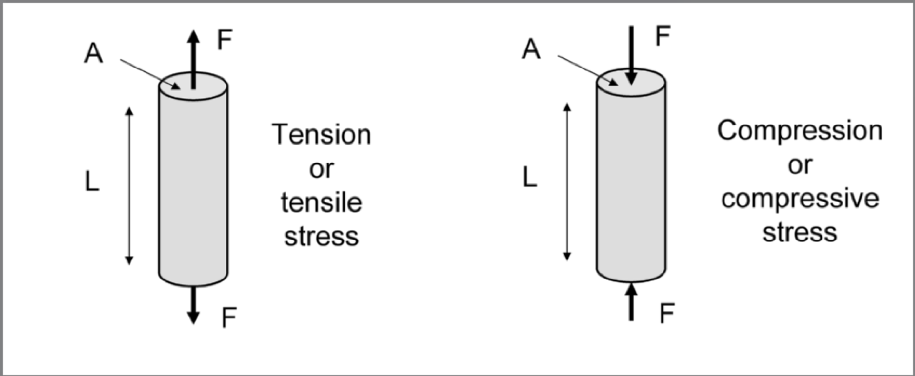
\includegraphics[width=0.5\linewidth]{img/lei_de_hooke_2} 

}

\caption{um cilindro de comprimento $L_0$ **(a)** a sofrer uma força de tracção **(b)** a sofrer uma força de     compressão.}\label{fig:img7}
\end{figure}

O módulo de Young tem unidades de \(N/m^2\) ou Pa (Pascal).
A relação linear entre a força aplicada e o deslocamento no comprimento do material é válida tanto na compressão como na tracção. O gráfico da figura \ref{fig:img8} mostra a relação entre o stress e a deformação do material. Na fase inicial do gráfico, a relação entre stress e deformação é linear e tem-se uma recta até ao ponto limite de linearidade. Até este ponto diz-se que o material comporta-se como um material de Hooke e a deformação causada pelo stress e totalmente reversível, ou seja, depois e sofrer o stress o material volta ao seu estado original. Entre o ponto de limite de linearidade e o ponto de limite de elástico, o material deixa de se comportar como um material de Hooke porque a relação entre o stress e a deformação deixa de ser linear.

\begin{figure}

{\centering 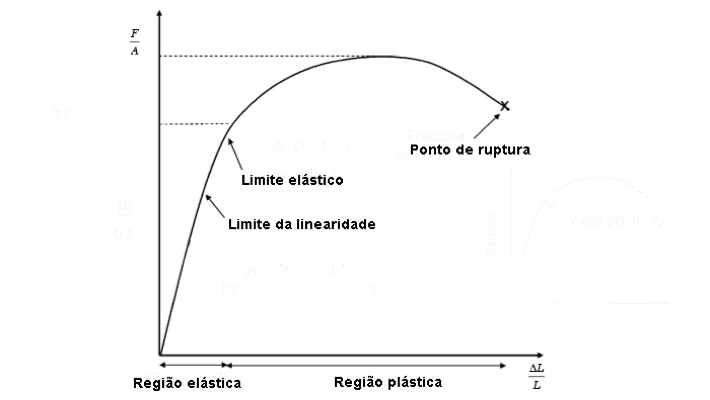
\includegraphics[width=0.5\linewidth]{img/lei_de_hooke_3} 

}

\end{figure}

Contudo, até ao limite elástico, o material volta ao seu estado original depois de sofrer o stress. Só quando o stress ultrapassa o limite elástico é que o material sofre deformação permanente e nunca mais volta a ter a sua forma original. A partir deste ponto diz-se que o material tem uma deformação permanente ou uma deformação plástica. No gráfico pode-se observar que a fronteira entre a região elástica e a região plástica do material é definida pelo ponto limite elástico.
Como vimos em cima, até ao limite elástico a deformação do material é totalmente reversível, contudo a relação entre stress e deformação não é a mesma quando o material volta ao seu formato original. Esta propriedade chama-se de resiliência. No gráfico da figura \ref{fig:img9} está representado o efeito de resiliência, que é a área azul. Esta área representa a energia térmica que é dissipada durante o processo de expansão e relaxamento do material.

\begin{figure}

{\centering 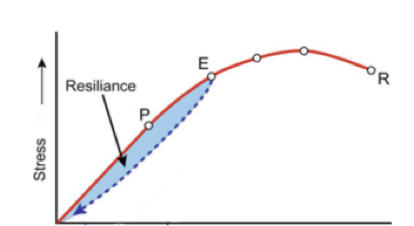
\includegraphics[width=0.5\linewidth]{img/lei_de_hooke_4} 

}

\end{figure}

\hypertarget{hidrostuxe1tica}{%
\chapter{Hidrostática}\label{hidrostuxe1tica}}

\hypertarget{introduuxe7uxe3o}{%
\section{Introdução}\label{introduuxe7uxe3o}}

A água está em toda parte, cobrindo 71\% da superfície da Terra. O conteúdo de água de um ser humano pode variar entre 45\% e 70\% do peso corporal. A água pode existir em três estados da matéria: sólido (gelo), líquido ou gasoso. A água flui através de rios, ribeiras, canais de irrigação e canos, para citar alguns. Os humanos tentaram controlar e aproveitar esse fluxo por meio de muitas tecnologias diferentes, como aquedutos, parafuso de Arquimedes, bombas e turbinas de água. A água no estado gasoso também flui. O vapor de água, mais leve que o ar, pode causar correntes de convecção que formam nuvens. No estado líquido, a densidade das moléculas de água é maior do que no estado gasoso, mas em ambos os estados a água pode fluir. A água líquida forma uma superfície, enquanto o vapor de água não. A água, tanto no estado líquido quanto gasoso, é classificada como fluido para distingui-la do estado sólido. Existe alguma ambiguidade no uso do termo fluido. O gelo flui num glaciar, mas muito lentamente. Portanto, por um curto intervalo de tempo em comparação com o intervalo de tempo envolvido no fluxo, o gelo glacial pode ser considerado um sólido. Na linguagem comum, o termo fluido é usado para descrever o estado líquido da matéria, mas um fluido é qualquer estado da matéria que flui quando há uma tensão de cisalhamento aplicada. A viscosidade de um fluido é uma medida da sua resistência à deformação gradual por tensão de cisalhamento ou tensão de tracção.

\hypertarget{densidade}{%
\section{Densidade}\label{densidade}}

A densidade de uma pequena quantidade de matéria é definida pela quantidade de massa \(\Delta M\) dividida pelo volume \(\Delta V\) desse elemento de matéria,

\begin{equation}
\rho=\frac{\Delta M}{\Delta V}
\label{eq:dens1}
\end{equation}

A unidade SI para a densidade é o kilograma por métro cúbico {[}\(kg/m^3\){]}. Se a densidade de um material é igual é todos os seus pontos, então a densidade é dada por

\begin{equation}
\rho=\frac{M}{V}
\label{eq:dens2}
\end{equation}

onde \(M\) é a massa do material e \(V\) é o volume do material. Um material com densidade constante é chamado de material \textit{homogéneo}. Para um material homogéneo, a densidade é uma propriedade intrínseca. Se dividirmos o matrerial é duas partes, a densidade será a mesma para as duas partes,

\begin{equation}
\rho=\rho_1=\rho_2
\label{eq:dens3}
\end{equation}

Contudo a massa e o volume são propriedades \textit{extrínsecas} do material. se dividirmos o material em duas partes, a massa total do material é a soma das massas das partes

\begin{equation}
M=M_1+M_2
\label{eq:dens4}
\end{equation}

tal como o volume

\begin{equation}
V=V_1+V_2
\label{eq:dens5}
\end{equation}

Na seguinte tabela podemos observar os valores da densidade de vários materiais.

\begin{table}

\caption{\label{tab:unnamed-chunk-4}Densidade de vários materiais}
\centering
\begin{tabular}[t]{l|l}
\hline
Material & Densidade, \$\textbackslash{}rho\$ [\$kg/m\textasciicircum{}3\$]\\
\hline
Hélio & \$0,179\$\\
\hline
Ar (ao nível do mar) & \$1,20\$\\
\hline
Esferovite & \$75\$\\
\hline
Madeira & \$0,7\textbackslash{}times 10\textasciicircum{}3\$\\
\hline
Etanol & \$0.81\textbackslash{}times 10\textasciicircum{}3\$\\
\hline
Gelo & \$0,92\textbackslash{}times 10\textasciicircum{}3\$\\
\hline
Água & \$1,0\textbackslash{}times 10\textasciicircum{}3\$\\
\hline
Água do mar & \$1,03\textbackslash{}times 10\textasciicircum{}3\$\\
\hline
Sangue & \$1,06\textbackslash{}times 10\textasciicircum{}3\$\\
\hline
Alumínio & \$2,7\textbackslash{}times 10\textasciicircum{}3\$\\
\hline
Ferro & \$7,87\textbackslash{}times 10\textasciicircum{}3\$\\
\hline
Cobre & \$8,94\textbackslash{}times 10\textasciicircum{}3\$\\
\hline
Chumbo & \$11,34\textbackslash{}times 10\textasciicircum{}3\$\\
\hline
Mercúrio & \$13,55\textbackslash{}times 10\textasciicircum{}3\$\\
\hline
Ouro & \$19,32\textbackslash{}times 10\textasciicircum{}3\$\\
\hline
Plutónio & \$19,84\textbackslash{}times 10\textasciicircum{}3\$\\
\hline
Ósmio & \$22,57\textbackslash{}times 10\textasciicircum{}3\$\\
\hline
\end{tabular}
\end{table}

\hypertarget{hidrodinuxe2mica}{%
\chapter{Hidrodinâmica}\label{hidrodinuxe2mica}}

\hypertarget{hemodinuxe2mica}{%
\chapter{Hemodinâmica}\label{hemodinuxe2mica}}

A hemodinâmica é o estudo da relação entre os factores físicos que afectam o fluxo sanguíneo através dos vasos. Neste capítulo, são discutidos esses factores e suas relações.

\hypertarget{o-fluxo-sanguuxedneo-uxe9-uma-funuxe7uxe3o-da-diferenuxe7a-de-pressuxe3o-e-resistuxeancia}{%
\section{O fluxo sanguíneo é uma função da diferença de pressão e resistência}\label{o-fluxo-sanguuxedneo-uxe9-uma-funuxe7uxe3o-da-diferenuxe7a-de-pressuxe3o-e-resistuxeancia}}

O fluxo sanguíneo (F) através de um vaso sanguíneo é determinado por dois factores principais: \textbf{(1)} diferença de pressão (\(\Delta\)P) entre as duas extremidades do vaso e \textbf{(2)} a resistência (R) ao fluxo sanguíneo através do vaso (Fig.\ref{fig:imghemo1}).

\begin{figure}

{\centering 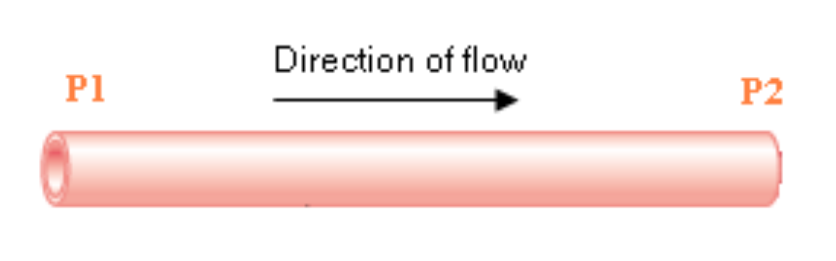
\includegraphics[width=0.5\linewidth]{img/hemo_1} 

}

\caption{Fluxo do sangue num vaso}\label{fig:imghemo1}
\end{figure}

A equação que relaciona estes parâmetros é
\begin{equation}
F=\frac{\Delta P}{R}
\label{eq:darcy}
\end{equation}

Esta equação é chamada de lei de Darcy ou lei de Ohm.

O fluxo (F) é definido como o volume de sangue que passa por cada ponto do vaso numa unidade de tempo. Normalmente, o fluxo sanguíneo é expresso em mililitros por minuto ou litros por minuto, mas também é expresso em mililitros por segundo.

A pressão, que é a força que empurra o sangue através do vaso, é definida como a força exercida numa superfície unitária da parede do tubo perpendicular ao fluxo. A pressão é expressa em milímetros de mercúrio (mmHg). Uma vez que a pressão muda ao longo do curso do vaso sanguíneo, não há uma única pressão a ser usada; portanto, o parâmetro de pressão utilizado é a diferença de pressão (\(\Delta P\)), também chamada de gradiente de pressão, que é a diferença entre a pressão no início do vaso (P1) e a pressão no final do vaso (P2), ou seja, fluxo de sangue (F) através de um vaso sanguíneo é determinado por dois factores principais: (1) diferença de pressão (\(\Delta P\)) entre as duas extremidades do vaso e (2) a resistência (R) ao fluxo sanguíneo através do vaso (Fig. \ref{fig:imghemo1}), ou seja, \(\Delta P = P1 - P2\).

Conforme visto na lei de Darcy, \(\Delta P\) é a causa do fluxo; sem diferença de pressão, não haveria fluxo. A energia da pressão é produzida pelo ventrículo e vai caindo ao longo do vaso devido à resistência. Noutras palavras, a resistência é a causa da queda de pressão ao longo de um vaso.
A resistência é o quão difícil é para o sangue fluir do ponto 1 ao ponto 2. A resistência impede o fluxo e é uma medida das interacções entre as partículas que fluem (incluindo moléculas e iões) e as interacções entre as partículas que fluem e a parede do vaso; quanto maior a resistência, menor o fluxo. Se a resistência for \(\infty\) (bloqueio completo do vaso) não haverá fluxo. A equação da resistência é:

\begin{equation}
R=\frac{8}{\pi}\frac{\eta L}{r^4}
\label{eq:resis}
\end{equation}

onde \(\eta=\) viscosidade, \(L=\) comprimento do vaso e \(r=\) raio interior do vaso

A viscosidade representa as interacções entre próprias partículas no fluxo, e o raio representa as interacções entre as partículas no fluxo e a parede do vaso. As unidades de viscosidade são \(Pa.s = Ns / m^2\), ou Poise (\(dynes.s / cm^2\)), com \(1 Pa.s = 10\) Poise.

Os glóbulos vermelhos, eritrócitos (hemácias), constituem 99\% do volume das partículas em suspensão do sangue. Portanto, a viscosidade do sangue depende da concentração de vários constituintes do plasma e da percentagem do volume dos glóbulos vermelhos (hematócrito), bem como do tamanho, forma e deformabilidade dos eritrócitos. Num indivíduo saudável todos estes parâmetros são constantes, portanto a viscosidade do sangue é constante e a viscosidade não é um meio de controle (regulação) da resistência. Em situações anormais, a viscosidade afecta anormalmente a resistência total. O hematócrito baixo, como na anemia, diminui a viscosidade do sangue. Inversamente, a policitemia aumenta a viscosidade e diminui o fluxo sanguíneo. Na anemia falciforme, os eritrócitos são deformados e inflexíveis, causando graves distúrbios do fluxo sanguíneo regional.
Na equação de resistência, \(L\) representa o comprimento do vaso. Como o comprimento dos vasos do corpo é constante, \(L\) não poderia ser usado para controlar a resistência.
A resistência tem relação inversa com a 4ª potência de \(r\) (raio interno do vaso); como tal, o raio do vaso tem o efeito mais poderoso sobre a resistência, significando que, com pequenas mudanças no raio, a resistência mudará dramaticamente. O raio é o principal factor de controle da resistência do sistema cardiovascular. O raio dos vasos do corpo é controlado pelo sistema simpático.
A resistência está localizada principalmente nas arteríolas. Assumindo um raio aórtico de \(15\) mm e um comprimento (arbitrário) de \(50\) cm e uma arteríola com um raio de 7,5 \(\mu m\) e um comprimento de 1 mm. A proporção do raio é de 2.000 e a proporção do comprimento é de \(\sim\) 500, portanto, a proporção de resistência seria \((2.000)^4/500\), ou seja, \(\sim 3\times10^{10}\). Isso significa que a resistência de uma única arteríola é \(3\times10^{10}\) tão grande quanto a de uma aorta de 50 cm de comprimento. Uma vez que existem \(3\times10^8\) arteríolas paralelas, sua resistência total é cerca de \(3\times10^{10}/3\times10^8 \cong 100\) vezes maior que a resistência da aorta (Westerhof et al.~2010).

Embora todos os vasos, excepto metarteríolas e capilares, sejam inervados pelo sistema simpático, as arteríolas recebem as inervações mais profundas e desempenham o papel principal no controle da resistência periférica total pelo sistema simpático.
A resistência de qualquer vaso pode ser calculada tendo \(\Delta P\) e \(F\). Para circulação sistémica, se a pressão aórtica média (P1) for considerada 100 mmHg e a pressão arterial direita média (P2) for 0 mmHg, a diferença de pressão (\(\Delta P\)) é 100 mmHg. Com um débito cardíaco de 6 l/min (100 ml/s), a resistência total é 100/100 = 1 mmHg/ml/s. Esta unidade é chamada de unidade de resistência periférica (PRU). Outras unidades físicas são utilizadas na clínica e a resistência é expressa em \(dyn.s.cm^5\) ou \(Pa.s/m^3\). A resistência periférica total da circulação sistémica pode mudar de 4 PRU em constrição muito forte para 0,2 PRU em grande dilatação dos vasos. No sistema pulmonar, a pressão arterial pulmonar média é 16 mmHg e a pressão arterial esquerda média é 2 mmHg, resultando em um \(\Delta P\) de 14 mm. Com um débito cardíaco de 100 ml/s, a resistência vascular pulmonar total é de 0,14 PRU, cerca de um sétimo daquela na circulação sistémica.
No corpo, os vasos sanguíneos estão dispostos em série e em paralelo. As artérias, arteríolas, capilares, vénulas e veias são organizadas em série. A resistência total de uma série de vasos é igual à soma das resistências de cada vaso:

\begin{equation}
R_{total}=R_1+R_2+R_3+...
\label{eq:resserie}
\end{equation}

Os vasos sanguíneos ramificam-se extensivamente para formar circuitos paralelos em todos os órgãos e tecidos do corpo. A resistência total dos vasos paralelos é calculada por:

\begin{equation}
\frac{1}{R_{total}}=\frac{1}{R_1}+\frac{1}{R_2}+\frac{1}{R_3}+...
\label{eq:respara}
\end{equation}

Como resultado, adicionar um vaso paralelo a um circuito reduzirá a resistência total. Esta é a razão pela qual a resistência de cada órgão sozinho é muito maior do que a resistência periférica total. Por exemplo, na circulação renal, se a pressão sanguínea na artéria renal for considerada 100 mmHg e a da veia renal for 10 mmHg e o fluxo renal for considerado como 20 ml/s (1200 ml/min), então R = 90/20 = 4,5 PRU, 4,5 vezes mais que a resistência total da circulação sistÉmica.

\hypertarget{lei-de-poisseuille}{%
\section{Lei de Poisseuille}\label{lei-de-poisseuille}}

Na equação \$F=\Delta P/R \$ substituirmos \(R\) pela sua equação, obtemos:

\begin{equation}
F=\frac{\pi \Delta P r^4}{8 \eta L}
\label{eq:pois}
\end{equation}

Esta equação é chamada de lei de Poiseuille. Como se poder observar, o fluxo é proporcional a \(\Delta P\), que é a principal causa do fluxo. O fluxo também é proporcional à 4ª potência do raio interno do vaso indicando a grande importância do raio para o fluxo.

\hypertarget{aplicauxe7uxf5es-fisioluxf3gicas-e-clinicas-da-lei-de-darcy}{%
\section{Aplicações fisiológicas e clinicas da lei de Darcy}\label{aplicauxe7uxf5es-fisioluxf3gicas-e-clinicas-da-lei-de-darcy}}

Na equação \(F = \Delta P/R\) se P1 é aumentado, uma vez que \(\Delta P = P1 - P2\), \(\Delta P\) aumentará o que resulta num aumento no fluxo sanguíneo (F) e (\(P_2\)). Por exemplo, durante o exercício, a contratilidade do ventrículo esquerdo aumenta e produz mais energia de pressão que resulta no aumento da pressão aórtica (\(P_1\)), fazendo com que o fluxo sanguíneo para vários órgãos e a pressão capilar (\(P_2\)) aumentem. Ao contrário, uma diminuição de (\(P_1\)) resulta numa diminuição do fluxo e da pressão capilar.

Um aumento na (\(P_2\)) resulta numa diminuição da \(\Delta P\) e do fluxo sanguíneo. Por exemplo, se a resistência venosa aumentar ou a pressão arterial (\(P_2\)) aumentar, como na insuficiência cardíaca, o \(\Delta P\) será menor do que o normal e o fluxo sanguíneo diminuirá. Isso subsequentemente resulta num pequeno aumento na pressão arterial (\(P_1\)). Portanto, uma mudança em qualquer uma das (\(P_1\)) ou (\(P_2\)) causa uma mudança semelhante na \(P\) correspondente, que é menor do que a primeira. É menor, porque a resistência causa sempre uma queda de pressão entre os dois pontos do vaso. Por exemplo, \(\uparrow P_1 \to \uparrow \Delta P(1º) \to \uparrow F \to \uparrow P_2 \to \downarrow \Delta P (2º)\), mas o fluxo é ainda maior, pois devido à resistência, a magnitude do aumento de \(P_2\) é menor que o aumento de \(P_1\), portanto, a magnitude da segunda mudança (diminuição) de \(\Delta P\) é menor do que a primeira mudança (aumento) de \(\Delta P\).

Alterar a resistência ajustando o raio dos vasos é o principal mecanismo de controle do fluxo sanguíneo para cada tecido e órgão, denominado controle local do fluxo sanguíneo. É também um dos dois principais mecanismos (controle do coração e resistência) para controlar a pressão arterial.

A equação de Darcy (\(F = \Delta P / R\)) poderia ser reescrita como: \(\Delta P = P1- P2 = FR\). Se \(R\) for aumentado diminuindo o raio, outros três parâmetros da equação serão alterados. A primeira coisa que acontece é a redução do fluxo, exactamente como esperado da equação de Darcy. A redução do fluxo causa um acumular de volume de sangue antes da resistência e uma diminuição no volume de sangue após a resistência; assim, \(P_1\) aumentará e \(P_2\) diminuirá e, subsequentemente, \(\Delta P\) ficará maior, exactamente como esperado da 2ª forma da equação de Darcy. O aumento resultante em \(\Delta P\) é sempre quantitativamente menor do que o aumento primário de \(R\); então, \(F\) é sempre menor do que antes. As etapas podem ser resumidas da seguinte forma:

\[R\uparrow \Rightarrow F\downarrow = \Delta P/R \uparrow \Rightarrow P_1\uparrow \& \hspace{0.1cm} P_2 \downarrow \Rightarrow \Delta P \uparrow \Rightarrow F\downarrow = \Delta P \uparrow /R \uparrow\]

Exactamente o oposto acontecerá se \(R\) for diminuído. Como já vimos, qualquer mudança em \(R\) mudará \(P_1\) e \(P_2\) em posições opostas. Por exemplo, quando alguém gira a válvula de uma torneira no sentido horário, o raio da saída diminui, o fluxo diminui, a pressão de saída (\(P_2\)) diminui e a pressão da água pré-válvula (\(P_1\)) aumenta.
Com base na lei de Darcy, se o sistema cardiovascular for aumentar o fluxo sanguíneo, ele pode aumentar \(\Delta P\) aumentando o trabalho cardíaco ou diminuir \(R\) diminuindo o fluxo simpático para os vasos, especialmente para as arteríolas, resultando numa diminuição da resistência. Também pode fazer as duas coisas (\(\Delta P \uparrow\) e \(R\downarrow\)). No mecanismo de controle local, apenas a resistência local é ajustada para controlar o fluxo sanguíneo para um tecido. O alto metabolismo de um tecido altera a concentração de alguns factores químicos, incluindo o oxigeno. Esses factores fazem com que as metarteríolas e os esfíncteres pré-capilares se dilatem. Com base na lei de Darcy, o fluxo sanguíneo para o tecido aumenta de modo que o fornecimento de sangue para o tecido seja proporcional ao seu metabolismo.
Quando a pressão arterial está baixa, o barorreflexo estimula o coração aumentando a contratilidade e a frequência cardíaca, o que resulta em \(P_1\) mais alto. Barorreflexo também aumenta a resistência periférica total, o que resulta numa maior \(P_1\)

A resistência causa queda de pressão em todo o sistema vascular (fig.~\ref{fig:imghemo2})). Nas grandes artérias, a resistência é relativamente pequena e a queda de pressão é pequena. As pequenas artérias têm resistência moderada ao fluxo sanguíneo. A resistência é maior nas arteríolas, que às vezes são chamadas de torneiras do sistema vascular. Portanto, a queda de pressão é maior na parte terminal das pequenas artérias e nas arteríolas (fig.~\ref{fig:imghemo2})).

Os vasos de resistência fazem queda de pressão de \$\sim\$100 a 30 mmHg. Com base na lei de Darcy, a alta resistência desses vasos aumenta a \(P_1\) (pressão arterial) e diminui a \(P_2\) (pressão capilar). Ambos os efeitos são absolutamente necessários para a sobrevivência. A pressão arterial elevada permite que o sangue chegue a todas as partes do corpo, especialmente à cabeça, que está em um nível mais alto do que o coração. O segundo efeito, pressão capilar baixa, também é muito útil porque evita que os capilares sejam danificados e é necessário para o transporte estável entre os capilares e o fluido intersticial. A alta pressão capilar torna os capilares muito permeáveis para que as proteínas possam atravessar o endotélio, o que resulta em edema.

\begin{figure}

{\centering 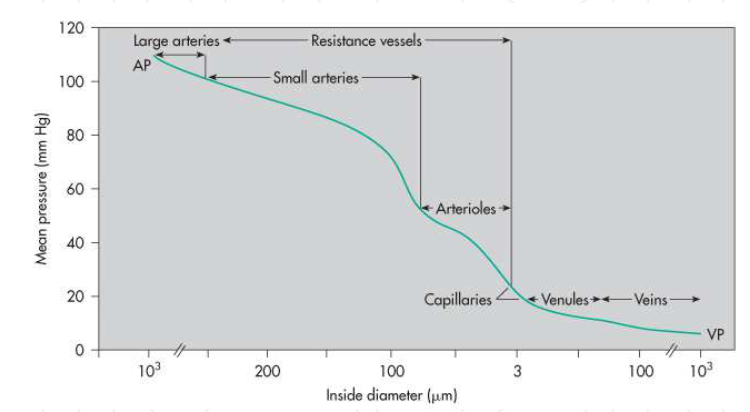
\includegraphics{img/hemo_2} 

}

\caption{Queda de pressão em todo o sistema vascular. AP, pressão arterial média; VP, pressão venosa}\label{fig:imghemo2}
\end{figure}

A anafilaxia é uma condição alérgica em que o débito cardíaco e a pressão arterial diminuem drasticamente. Resulta de uma reacção antígenio-anticorpo depois que um antígenio ao qual a pessoa é sensível entra na circulação, causando a secreção de histamina por basófilos e mastócitos. A histamina dilata as arteríolas, resultando em grande redução da pressão arterial que pode resultar em coma e morte. Drogas vasodilatadoras em excesso também podem produzir efeito semelhante.
Num aneurisma, parte de uma artéria dilata-se anormalmente. Com base na lei de Darcy, o fluxo sanguíneo para a zona perfundida por essa artéria é aumentado (\(F \uparrow\)), o que resulta em uma pressão mais alta na microcirculação dessa zona (\(P_2 \uparrow\)), o que pode produzir dor e danos.

Na coarctação da aorta descendente (condição médica na qual a aorta é estreita desde o nascimento), causa estreitamento do lúmen. Como esperado pela lei de Darcy, o fluxo sanguíneo para as partes inferiores do corpo está seriamente diminuído (\(F \downarrow\)). Como consequência, a pressão arterial na parte inferior da aorta diminui (\(P_2 \downarrow\)) e na parte superior da aorta pode ser 40-50 por cento maior (\(P_1 \uparrow\)) do que na aorta inferior. Devido à baixa pressão arterial renal, ocorre retenção de água e sal que vai levar, eventualmente, a pressão arterial da parte inferior do corpo ao normal e produzir hipertensão na parte superior do corpo.

Nas doenças isquêmicas do coração, o estreitamento ou obstrução de uma ou mais artérias coronárias diminui ou cessa o fluxo sanguíneo para as regiões abastecidas pelas artérias afetadas.

Na estenose aórtica, o diâmetro da abertura da válvula aórtica é reduzido significativamente, e a pressão de pulso aórtica (diferença entre a pressão sistólica e diastólica) é reduzida significativamente devido à grande diminuição da pressão sistólica. Com base na lei de Darcy, devido à alta resistência da válvula aórtica, \(P_1\) (pressão ventricular) aumenta e \(P_2\) (pressão sistólica aórtica) diminui. Isso é exactamente o que vemos na doença. Devido à alta pressão ventricular, pode ocorrer hipertrofia ventricular.

A enxaqueca é um complexo de sintomas de dores de cabeça periódicas, frequentemente com irritabilidade, náuseas, vómitos, prisão de ventre ou diarreia e fotofobia. É precedido por constrição de algumas artérias cranianas, o que resulta em baixo fluxo sanguíneo para as regiões afectadas e, consequentemente, resulta em sintomas prodrómicos, especialmente sintomas oculares. Em seguida, ocorre uma vasodilatação notável dessas artérias cranianas, resultando em hiperperfusão das regiões afectadas, que produz outros sintomas, especialmente dor de cabeça.

\hypertarget{fluxo-laminar-e-turbulento}{%
\section{Fluxo laminar e turbulento}\label{fluxo-laminar-e-turbulento}}

O fluxo sanguíneo nos vasos rectos é normalmente laminar. O sangue move-se em suaves camadas concêntricas paralelas. Conforme o fluxo aumenta, o movimento do fluido torna-se ondulado, levando a vórtices em diferentes direções aparentemente aleatórias. Esse movimento irregular do fluido é chamado de turbulência (Fig. \ref{fig:imghemo3})).

\begin{figure}

{\centering 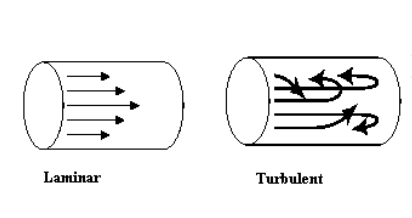
\includegraphics{img/hemo_3} 

}

\caption{Fluxo laminar e turbulento}\label{fig:imghemo3}
\end{figure}

No fluxo turbulento a resistência ao fluxo é maior e energeticamente mais dispendiosa do que o laminar, pois parte da energia mecânica é perdida no movimento errático entre as partículas do fluido. A probabilidade de turbulência está relacionada à densidade do sangue, velocidade, diâmetro do vaso e viscosidade do sangue. Para julgar se um fluxo de fluido é laminar ou turbulento, o número de Reynolds (Re, um parâmetro adimensional: não tem unidade) é frequentemente usado. Re é definido como:

\begin{equation}
R_e=\frac{\rho v D}{\eta}
\label{eq:reynolds}
\end{equation}

onde \(\rho\) é a densidade do fluido, \(v\) é a velocidade do fluido, \(D\) é o raio interno do tubo e \(\eta\) é a viscosidade do fluido. O número de Reynolds reflecte o rácio entre a inércia e os efeitos da viscosidade. O número Reynolds crítico é 2200. Para números de Reynolds baixos (\textless2200), os efeitos viscosos são dominantes e o fluxo é laminar, mas para números de Reynolds altos (\textgreater{} 2200), o fluxo é turbulento. Para números de transição em torno do número Reynolds crítico de 2200, o fluxo não é estritamente laminar nem estritamente turbulento.

Em condições normais de repouso, os fluxos arteriais são laminares. Mas em exercícios pesados, onde o fluxo pode aumentar até cinco vezes, o número de Reynolds pode ficar maior do que o valor crítico e ocorrer turbulência.

O fluxo laminar pode ser perturbado nos pontos de ramificação das artérias, resultando em turbulência que pode depositar as placas ateroscleróticas.

A turbulência ocorre menos na aceleração do fluxo, enquanto que pode ocorrer mais rapidamente na desaceleração dos fluxos. Por exemplo, a turbulência ocorre no ponto distal a uma estenose. As partículas de fluido aceleram através da parte estreita da estenose e desaceleram rapidamente na parte após as estenose, em expansão, resultando em turbulência. A turbulência na estenose grave pode ser iniciada para números de Reynolds tão baixos quanto 50 (Westerhof et al.~2010, p-23). Essa turbulência também alarga o vaso após a estenose. Da mesma forma, a constrição de uma artéria produz turbulência e som. Esta é a razão pela qual os sopros são ouvidos nas artérias contraídas por placas ateroscleróticas e os sons de Korotkoff ouvidos durante a medição da pressão arterial (Barrett et al.~2010, p-540). Na anemia grave, devido à baixa viscosidade, sopros cardíacos funcionais são frequentemente ouvidos.

\hypertarget{principio-de-bernoulli}{%
\section{Principio de Bernoulli}\label{principio-de-bernoulli}}

Em relação à lei de Darcy, alguns aspectos da hemodinâmica podem parecer estranhos. Por exemplo, a pressão arterial média da aorta é de cerca de 100 mmHg, enquanto é de 180 mmHg nas artérias do pé quando um pessoa está em pé. A pressão arterial muito alta do pé deve-se à força gravitacional, já que uma coluna de sangue com uma altitude de \$\sim\$130 cm produz uma pressão alta nas artérias do pé. Com base na lei de Darcy, uma vez que a pressão nas artérias do pé é maior do que na aorta, o sangue deveria subir das artérias do pé para a aorta, o que não acontece. Além disso, a pressão arterial nos seios venosos do cérebro é altamente negativa, enquanto a pressão do átrio direito é \$\sim\$0. Novamente com base na lei de Darcy, o sangue deve se mover para cima, do átrio direito para o sistema venoso do cérebro, o que não é o caso. Esses problemas são resolvidos pelo princípio de Bernoulli. A teoria de Bernoulli afirma que o fluxo entre os pontos A e B depende da diferença de energia mecânica total entre A e B, não apenas da diferença de pressão. A energia mecânica total consiste em energia de pressão, energia potencial e energia cinética. A energia da pressão é igual à pressão \(\times\) volume (P \(\times\) V). A energia potencial é igual à massa do fluido (m) \(\times\) força gravitacional (g) \(\times\) altura (h) . a Energia cinética é igual à massa (m) \(\times\) velocidade ao quadrado (\(v^2\)) dividido por 2 (\(m\times v^2/2\)). Então a

\begin{equation}
Energia \hspace{0.1cm}mecanica\hspace{0.1cm} total = PV + mgh + \frac{1}{2}mv^2
\label{eq:bernoulli}
\end{equation}

Com base nas condições, essas pressões podem ser facilmente convertidas umas nas outras. Por exemplo, considere o modelo apresentado na figura \ref{fig:imghemo4}). Nesta figura está uma experiência que mostra alguns pontos hidráulicos básicos. Nesta experiência, o fluxo no tubo é constante e é impulsionado pelo gradiente da energia mecânica total. Na primeira parte, a área da secção transversal (A) é 6 e a velocidade (v) é 1. Com base na equação V = F/A (V: velocidade, F: fluxo, A: área da secção transversal), como a área da secção transversal do meio do tubo fica menor, a velocidade aumenta com a mesma proporção.

\begin{figure}
\centering
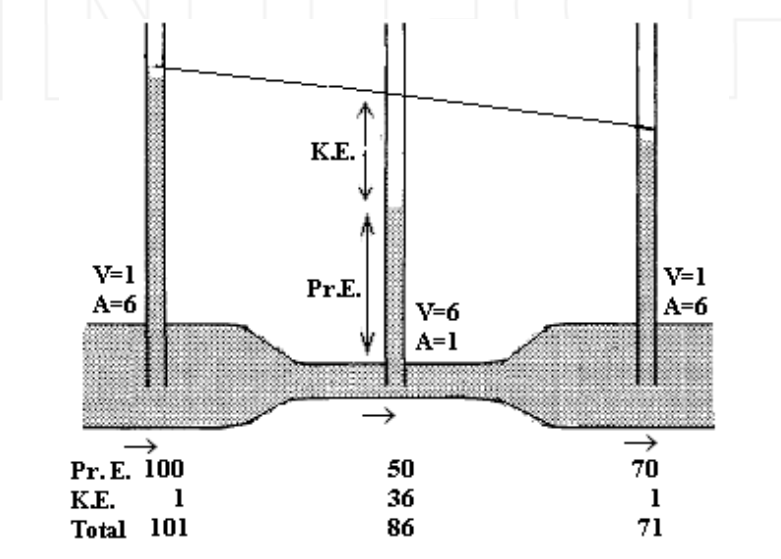
\includegraphics{img/hemo_4.png}
\caption{\label{fig:imghemo4}O fluxo é impulsionado pela diferença total de energia mecânica. No meio do tubo, a área da seção transversal (A) fica menor, resultando num aumento da velocidade (v). Por outras palavras, a energia da pressão é convertida em energia cinética. Na terceira parte do tubo, acontecerá o oposto. (Pr.E., energia da pressão; K.E., energia cinética.)}
\end{figure}

Isto significa que a energia da pressão é convertida em energia cinética. Isto é indicado pelos números na parte inferior da figura e no tubo vertical do meio. Uma vez que existem gradientes mecânicos e de pressão, o fluxo da primeira parte para a segunda parte do tubo é consistente com as equações de Darcy e de Bernoulli. A terceira parte do tubo ao ficar mais larga, resulta num aumento da energia de pressão e uma diminuição da energia cinética. Aqui, a energia cinética é convertida em energia de pressão. Isso mostra que essas três energias mecânicas podem ser facilmente convertidas uma na outra. O fluxo da parte do meio para a terceira parte não é esperado da lei de Darcy, mas é consistente com o princípio de Bernoulli. Outro ponto importante mostrado nesta experência é que, devido à resistência, a energia mecânica total diminui ao longo do tubo.

Agora podemos explicar os exemplos mencionados acima. Na postura erecta, o sangue aórtico possui muito mais energia potencial gravitacional do que as artérias do pé, de forma que a energia mecânica total na aorta é maior do que nas artérias do pé e faz com que o sangue flua da aorta para o pé.
Quando alguém se deita, a lei de Darcy é suficiente para explicar o fluxo sanguíneo, mas na posição sentada ou em pé, a energia potencial gravitacional é muito grande e a lei de Bernoulli deve ser aplicada para uma explicação mais precisa do fluxo sanguíneo. Por exemplo, na postura erecta, o fluxo sanguíneo para o pulmão não poderia ser bem explicado sem usar o princípio de Bernoulli. Como a pressão nas artérias pulmonares é baixa, a energia potencial gravitacional é comparativamente grande e afecta muito o fluxo sanguíneo pulmonar, de modo que, durante a diástole, o sangue não atinge o ápice do pulmão.

\hypertarget{lei-de-laplace}{%
\section{Lei de Laplace}\label{lei-de-laplace}}

A lei de Laplace fornece a relação entre a pressão transmural, a tensão da parede, o raio e a espessura da parede em um vaso (Fig. \ref{fig:imghemo5})) como:

\begin{equation}
T=\frac{P.r}{w}
\label{eq:laplace}
\end{equation}

Onde \(T\) é a força por unidade de comprimento tangencial à parede do vaso chamada tensão da parede (\(dynes/cm\)), \(P\) é a pressão transmural, pressão intravascular menos pressão extravascular, em \(dynes/cm^2\), \(r\) é o raio do vaso em \(cm\), e \(w\) é espessura do vaso em \(cm\).

\begin{figure}

{\centering 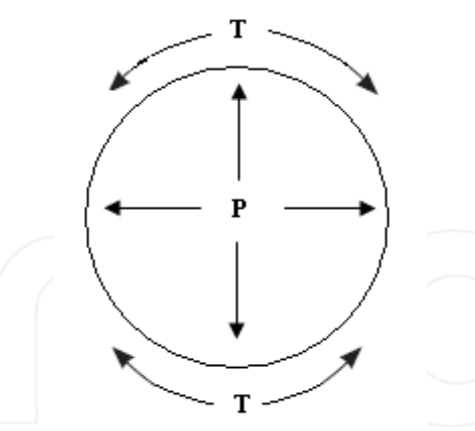
\includegraphics{img/hemo_5} 

}

\caption{Pressão transmural $P$ e tensão da parede $T$ num vaso}\label{fig:imghemo5}
\end{figure}

Os capilares de paredes finas podem suportar uma alta pressão sanguínea interna, pois embora a espessura da parede seja muito pequena, o raio também é muito pequeno e sua pressão interna é muito menor do que nas artérias. No aneurisma (alargamento local de uma artéria), como o raio fica maior, a pressão de distensão aumenta e torna o vaso mais vulnerável à ruptura. Na hipertrofia excêntrica, onde um ventrículo se dilata, devido ao aumento do raio, a força de distensão é maior e o ventrículo deve trabalhar mais para bombear o volume sistólico normal isso vai deteriorar ainda mais o ventrículo.

\hypertarget{a-velocidade-inversamente-relacionada-com-a-uxe1rea-da-seuxe7uxe3o-transversal}{%
\section{A velocidade inversamente relacionada com a área da seção transversal}\label{a-velocidade-inversamente-relacionada-com-a-uxe1rea-da-seuxe7uxe3o-transversal}}

A velocidade (\(V\)) está relacionada ao fluxo (\(F\)) e inversamente relacionada à área da seção transversal (\(A\)) de um vaso da seguinte forma:

\begin{equation}
V=\frac{F}{A}
\label{eq:velo}
\end{equation}

Como os vasos sanguíneos ramificam-se extensivamente da aorta para os capilares, a área de secção transversal de cada vaso diminui, enquanto a área da secção transversal total aumenta.

\begin{figure}

{\centering 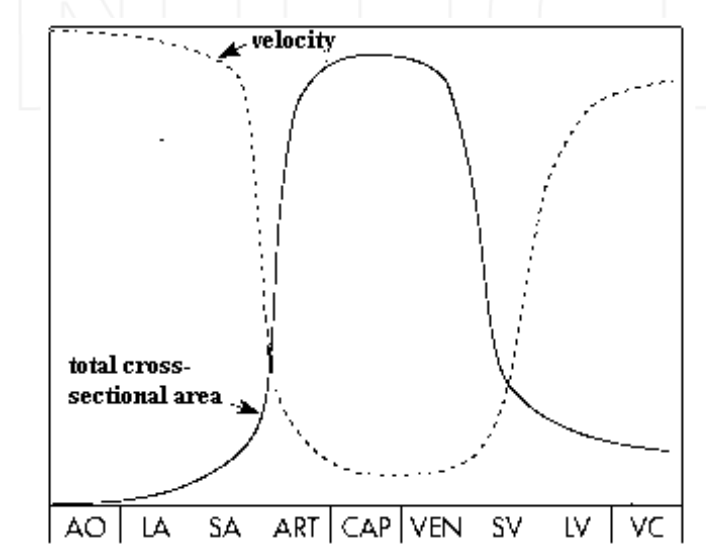
\includegraphics{img/hemo_6} 

}

\caption{Velocidade e área transversal total na circulação sistêmica. Existe a área transversal máxima e velocidade mínima nos capilares. AO, aorta; LA, grandes artérias; SA, pequenas artérias; ART, arteríolas; CAP, capilares; VEN, vênulas; SV, veias pequenas ; LV, veias grandes; VC, veia cava.}\label{fig:imghemo6}
\end{figure}

Os capilares têm a área transversal total máxima, resultando na menor velocidade do sangue (Fig. \ref{fig:imghemo6}). Essa velocidade baixa fornece tempo suficiente para a troca entre o sangue e o fluido intersticial

\hypertarget{elasticidade-e-complacuxeancia}{%
\section{Elasticidade e Complacência}\label{elasticidade-e-complacuxeancia}}

Quando uma barra de um material com área de secção transversal \(A\) e comprimento \(l_0\) é submetida a uma força (\(F\)), sofre uma alteração no comprimento de \(\Delta l\) (Fig. \ref{fig:imghemo7}). Para uma barra com uma área de secção transversal maior, a mesma força produzirá uma alteração menor no comprimento. Além disso, se o comprimento inicial (\(l_0\)) for mais longo, a mesma força causa uma alteração maior no comprimento. Para ter uma caracterização única do material, independente do comprimento e espessura da amostra, a força é normalizada começando na área da secção transversal, \(\sigma = F/A\) chamada tensão (ou stress), e o comprimento é normalizado pelo comprimento inicial \(\epsilon = \Delta l/ l_0\) chamado deformação. A elasticidade é definida como \(E = \sigma / \epsilon\)

\begin{figure}

{\centering 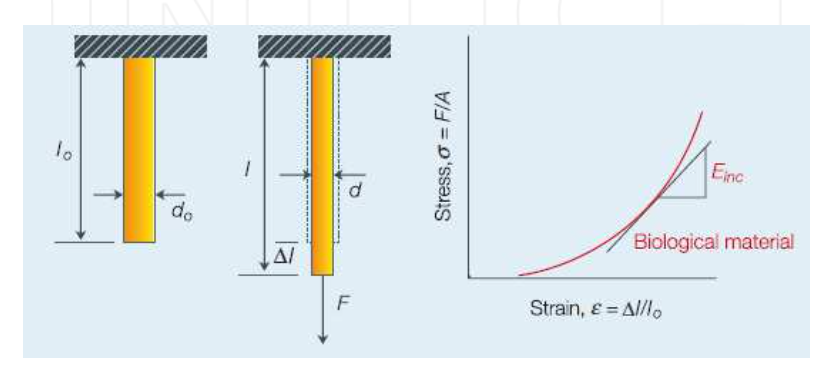
\includegraphics{img/hemo_7} 

}

\caption{Relação tensão-deformação para materiais biológicos}\label{fig:imghemo7}
\end{figure}

Para os vasos ou coração, aumentar o volume sanguíneo resulta num aumento na pressão interna e aumentar a pressão interna resulta num aumento do volume. A pressão é comparável ao stress e o volume é comparável à deformação. Portanto, na fisiologia cardiovascular, a relação pressão-volume (Fig. \ref{fig:imghemo8}) é normalmente usada em vez da relação stress-deformação. Uma vantagem da relação pressão-volume é que ela pode ser medida \(\textit{in vivo}\). É importante notar que a relação pressão-volume não caracteriza o material sozinho, mas inclui a estrutura do órgão como um todo. A mudança de volume por unidade de pressão é chamada complacência (\(C = \Delta V / \Delta P\)). A mudança de pressão por uma unidade de volume é chamada de elastância (\(E = \Delta P / \Delta V\)). Para órgãos biológicos como vasos e coração, a relação pressão-volume é uma curva em direcção ao eixo do volume indicando que ao aumentar o volume ou a rigidez, a pressão aumenta (Fig. \ref{fig:imghemo8}). Portanto, não há uma valor único de complacência ou elastância e para um ponto utiliza-se a tangente da curva pressão-volume.

\begin{figure}

{\centering 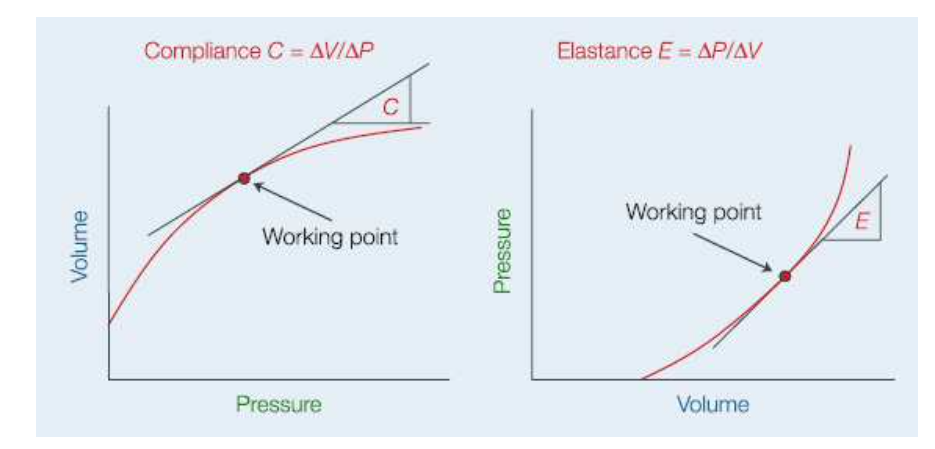
\includegraphics{img/hemo_8} 

}

\caption{Relação pressão-volume para órgãos biológicos}\label{fig:imghemo8}
\end{figure}

A complacência e a elastância dependem do volume original (\(V_0\)) do órgão em estudo. Para comparar as propriedades de diferentes vasos sanguíneos, a complacência e a elastância devem ser normalizadas em relação ao volume original do órgão. A complacência normalizada é chamada de distensibilidade {[}distensibilidade \(= C / V_0 = \Delta V / (\Delta P.V_0)\){]}. A elastância normalizada é chamada de elasticidade de volume {[}elasticidade de volume \(= E.V_0 = (\Delta P.V_0) / \Delta V\){]}.

\hypertarget{aplicauxe7uxf5es-cluxednicas-e-fisioluxf3gicas}{%
\section{Aplicações clínicas e fisiológicas}\label{aplicauxe7uxf5es-cluxednicas-e-fisioluxf3gicas}}

A distensibilidade das veias é 8 vezes maior do que as artérias e o volume original das veias é 3 vezes maior do que as artérias, portanto a complacência de cada veia é 24 vezes maior que a sua artéria correspondente (artéria e veia que têm o mesmo fluxo). Isso significa que a perfusão de uma veia, e da sua artéria correspondente, com o mesmo volume de sangue aumenta a pressão da artéria 24 vezes mais que na veia. Portanto, as veias podem armazenar grande quantidade de sangue com pouco aumento de pressão. As veias são chamadas de vasos de capacitância, armazenando 60-70 por cento do volume total de sangue.
A Figura \ref{fig:imghemo9}) mostra o efeito da pressão sanguínea no fluxo sanguíneo através de um vaso isolado. Conforme esperado pela lei de Darcy (\(F = \Delta P/R\)), o aumento da pressão resulta num aumento do fluxo, mas, na verdade, o efeito da pressão no fluxo sanguíneo é maior do que o esperado pela lei de Darcy (Fig. \ref{fig:imghemo9}b), conforme mostrado pela linhas curvas para cima na Figura \ref{fig:imghemo8}a. Isso porque, devido à distensibilidade vascular, o aumento da pressão arterial não só aumenta a força que empurra o sangue através dos vasos, mas também distende os vasos elásticos, diminuindo a resistência vascular. Portanto, a elasticidade faz com que o coração trabalhe menos para bombear o débito cardíaco normal, resultando numa sobrevida mais longa.

\begin{figure}

{\centering 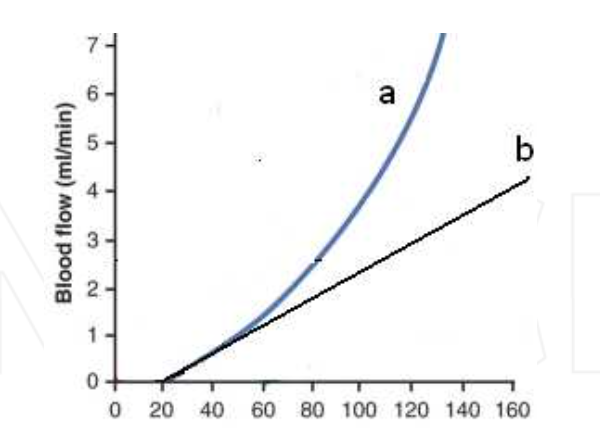
\includegraphics{img/hemo_9} 

}

\caption{Efeito da pressão sanguínea no fluxo sanguíneo através de um vaso isolado (a), e calculado a partir da lei de Darcy (b)}\label{fig:imghemo9}
\end{figure}

Na arteriosclerose, os vasos sanguíneos são menos distensíveis, o que resulta numa maior resistência, causando hipertensão, o que resulta num maior trabalho do coração. Estes sintomas têm efeitos graves de deterioração do sistema cardiovascular.

Durante a sístole, devido à distensibilidade vascular, a hipertensão arterial distende as artérias, ou seja, alguma energia da pressão é armazenada nas paredes das artérias como energia potencial. Durante a diástole, a parede das artérias retorna à sua posição diastólica, libertando a energia potencial armazenada para o sangue como energia de pressão. Esta função atenua a pressão sistólica e aumenta a pressão diastólica, resultando numa pressão arterial normal (diferença entre a pressão sistólica e a pressão diastólica) de 40 mmHg. Manter a pressão diastólica razoavelmente alta mantém o sangue fluindo durante a diástole. Na arteriosclerose, devido à rigidez das artérias, menos energia da pressão é armazenada na parede das artérias, fazendo com que a pressão sistólica fique anormalmente alta, resultando numa pressão arterial alta que tem um efeito de deterioração nas artérias.
Outro benefício fisiológico da elasticidade é o amortecimento da pressão arterial nas artérias menores, arteríolas e capilares. A Figura 10 mostra mudanças típicas na pressão arterial conforme o pulso viaja para os vasos periféricos. A intensidade da pulsação torna-se progressivamente menor nas artérias menores e, eventualmente, desaparece nos capilares. Na verdade, somente quando as pulsações aórticas são extremamente grandes ou as arteríolas muito dilatadas é que as pulsações nos capilares podem ser observadas. A falta de pulsação nos capilares garante pressão estável, portanto, permeabilidade estável e transporte estável através da parede dos capilares.

\begin{figure}

{\centering 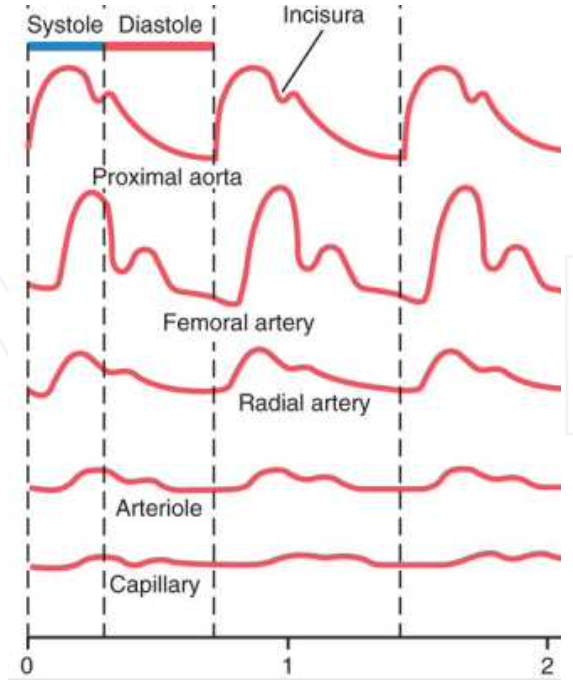
\includegraphics{img/hemo_10} 

}

\caption{Atenuação da pressão de arterial nas artérias menores, arteríolas e capilares}\label{fig:imghemo10}
\end{figure}

A causa da diminuição progressiva das pulsações na periferia é dupla: (1) resistência e (2) elasticidade dos vasos. A resistência é a causa da queda de pressão em todos os vasos, diminuindo assim a pressão arterial A elasticidade diminui continuamente a sístole e aumenta a pressão da diástole, aproximando-os um do outro.

  \bibliography{book.bib,packages.bib}

\end{document}
